\chapter{Multiple Integrals}
\label{chapter:mult-integrals}
%Begin Section 3.1
\section{Double Integrals}
In single-variable calculus, differentiation and integration are thought of as inverse operations. For instance, to
integrate a function $f(x)$ it is necessary to find the antiderivative of $f$, that is, another function $F(x)$
whose derivative is $f(x)$. Is there a similar way of defining integration of real-valued functions of two or
more variables? The answer is yes, as we will see shortly. Recall also that the definite integral of a
nonnegative function $f(x) \ge 0$ represented the area ``under'' the curve $y=f(x)$. As we will now see, the
\emph{double integral} of a nonnegative real-valued function $f(x,y) \ge 0$ represents the \emph{volume} ``under'' the
surface $z=f(x,y)$.\index{multiple integral}\index{integral!multiple}

Let $f(x,y)$ be a continuous function such that $f(x,y) \ge 0$ for all $(x,y)$ on the \textbf{rectangle}
$R = \lbrace (x,y): a \le x \le b ,\, c \le y \le d \rbrace$ in $\Real{2}$. We will often write this as
$R = \lbrack a,b \rbrack \times \lbrack c,d \rbrack$. For any number $x*$ in the interval $\lbrack a,b \rbrack$, slice
the surface $z=f(x,y)$ with the plane $x=x*$ parallel to the $yz$-plane.
Then the trace of the surface in that plane is the \emph{curve} $f(x*,y)$, where $x*$ is fixed and only $y$
varies. 
The area $A$ under that curve 
(that is, the area of the region between the curve and the $xy$-plane)
as $y$ varies over the interval $\lbrack c,d \rbrack$ then depends only on the value of $x*$. So using the variable $x$ instead of
$x*$, let $A(x)$ be that area (see Figure \ref{fig:iterint}).

\begin{figure}[h]
 \begin{center}
  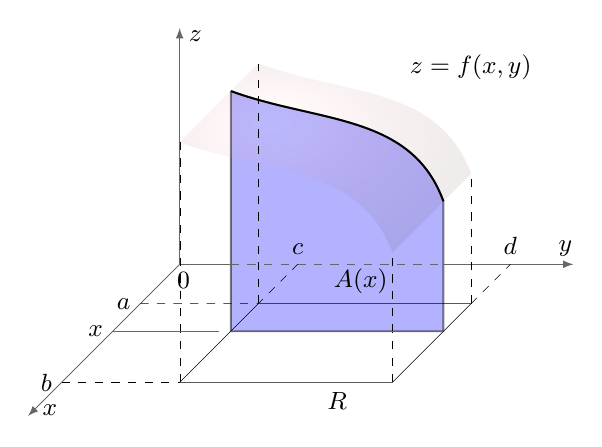
\begin{tikzpicture}
   \usetikzlibrary{arrows}
   \definecolor{planecolor}{HTML}{FFB270}
   \definecolor{surfcolor}{HTML}{006146}
   \filldraw [opacity=0.5,fill=blue!60,line width=0.7pt] (0.65,2.2) to[out=-20,in=110] (3.35,0.8) -- (3.35,-0.85) --
    (0.65,-0.85) -- (0.65,2.2);
   \shade [opacity=0.1,ball color=red!40] (0,1.55) to[out=-20,in=110] (2.7,0.15) -- (3.7,1.15) to[out=110,in=-20]
    (1,2.55) -- (0,1.55);
   \draw [black!60,line width=0.3pt] (0,0) -- (0.65,0,0);
   \draw [dashed,black!60,line width=0.3pt] (0.65,0) -- (3.35,0,0);
   \draw [black!60,line width=0.3pt,-latex] (3.35,0) -- (5,0,0);
   \draw [black!60,line width=0.3pt,-latex] (0,0) -- (0,3,0);
   \draw [black!60,line width=0.3pt,-latex] (0,0) -- (0,0,5);
   \pgfputat{\pgfpointxyz{4.9}{0.2}{0}}{\pgfbox[center,center]{\small $y$}};
   \pgfputat{\pgfpointxyz{0.2}{2.9}{0}}{\pgfbox[center,center]{\small $z$}};
   \pgfputat{\pgfpointxyz{0.2}{0}{4.8}}{\pgfbox[center,center]{\small $x$}};
   \pgfputat{\pgfpointxyz{0.05}{-0.2}{0}}{\pgfbox[center,center]{\small $0$}};
   \draw [dashed,line width=0.2pt] (-0.5,-0.5) -- (1,-0.5) --(1.5,0);
   \draw [dashed,line width=0.2pt] (-1.5,-1.5) -- (0,-1.5);
   \draw [dashed,line width=0.2pt] (3.7,-0.5) -- (4.2,0);
   \draw [line width=0.2pt] (1,-0.5) -- (3.7,-0.5) -- (2.7,-1.5) -- (0,-1.5) -- (1,-0.5);
   \draw [dashed,line width=0.1pt] (0,-1.5) -- (0,1.55);
   \draw [dashed,line width=0.1pt] (1,-0.5) -- (1,2.55);
   \draw [dashed,line width=0.1pt] (3.7,-0.5) -- (3.7,1.15);
   \draw [dashed,line width=0.1pt] (2.7,-1.5) -- (2.7,0.15);
   \node [above] at (2.3,-0.5) {\small $A(x)$};
   \node [below] at (2.0,-1.5) {\small $R$};
   \draw [black!60,line width=0.1pt] (-0.85,-0.85) -- (0.5,-0.85);
   \draw [black!60,line width=0.1pt] (0.65,-0.85) -- (3.35,-0.85);
   \draw [line width=0.7pt] (0.65,2.2) to[out=-20,in=110] (3.35,0.8);
   \node [left] at (-0.5,-0.5) {\small $a$};
   \node [left] at (-0.85,-0.85) {\small $x$};
   \node [left] at (-1.5,-1.5) {\small $b$};
   \node [above] at (1.5,0) {\small $c$};
   \node [above] at (4.2,0) {\small $d$};
   \node [right] at (2.8,2.5) {\small $z = f(x,y)$};
  \end{tikzpicture}
 \end{center}
 \caption[]{\quad The area $A(x)$ varies with $x$}
 \label{fig:iterint}
\end{figure}

Then $A(x) = \int_c^d f(x,y)\,dy$ since we are treating $x$ as fixed, and only $y$ varies. This makes sense since
for a fixed $x$ the function $f(x,y)$ is a continuous function of $y$ over the interval $\lbrack c,d \rbrack$, so
we know that the area under the curve is the definite integral. The area $A(x)$ is a function of $x$, so by the
``slice'' or cross-section method from single-variable calculus we know that the volume $V$ of the \emph{solid} under
the surface $z=f(x,y)$ but above the $xy$-plane over the rectangle $R$ is the integral over $\lbrack a,b \rbrack$ of
that cross-sectional area $A(x)$:
\begin{equation}\label{eqn:voliterx}
 V ~=~ \int_a^b A(x)\,dx ~=~ \int_a^b \left[ \int_c^d f(x,y)\,dy \right] \,dx
\end{equation}
We will always refer to this volume as ``the volume under the surface''.
The above expression uses what are called \textbf{iterated integrals}. First the function $f(x,y)$ is integrated as a
function of $y$, treating the variable $x$ as a constant (this is called \emph{integrating with respect to $y$}). That
is what occurs in the ``inner'' integral between the square brackets in equation (\ref{eqn:voliterx}). This is the
first iterated integral.\index{integral!iterated}
Once that integration is performed, the result is then an expression involving only $x$, which can then be
\emph{integrated with respect to $x$}. That is what occurs in the ``outer'' integral above (the second iterated
integral). The final result is\index{double integral}\index{iterated integral}\index{integral!double}
then a number (the volume). This process of going through two iterations of integrals is called \emph{double
integration}, and the last expression in equation (\ref{eqn:voliterx}) is called a \textbf{double integral}.

Notice that integrating $f(x,y)$ with respect to $y$ is the inverse operation of taking the partial
derivative of $f(x,y)$ with respect to $y$. 

Also, we could have taken the area of cross-sections under
the surface which were parallel to the $xz$-plane, which would then depend only on the variable $y$, so that the volume would be
\begin{equation}\label{eqn:volitery}
 V ~=~ \int_c^d \left[ \int_a^b f(x,y)\,dx \right] \,dy ~.
\end{equation}
It turns out that in general\footnote{due to \emph{Fubini's Theorem}. See Ch. 18 in \cite{tm}.} the order of the
iterated integrals does not matter. Also, we will usually discard the brackets and simply write
\begin{equation}\label{eqn:volint}
 V ~=~ \int_c^d \int_a^b f(x,y)\,dx \,dy ~,
\end{equation}
where it is understood that the fact that $dx$ is written before $dy$ means that the function $f(x,y)$ is first
integrated with respect to $x$ using the ``inner'' limits of integration $a$ and $b$, and then the resulting function
is integrated with respect to $y$ using the ``outer'' limits of integration $c$ and $d$. This order of integration can
be changed if it is more convenient.\index{$\iint$}

\medskip
\hrule width \textwidth height 0.5pt
\begin{exmp}\label{exmp:volplane}
 Find the volume $V$ under the plane $z=8x+6y$ over the rectangle $R = \lbrack 0,1 \rbrack \times \lbrack 0,2 \rbrack$.
 \smallskip
 \par\noindent \emph{Solution:} We see that $f(x,y)=8x+6y \ge 0$ for $0 \le x \le 1$ and $0 \le y \le 2$, so:
 \begin{align*}
  V ~&=~ \int_0^2 \int_0^1 (8x+6y)\,dx \,dy\\
   &=~ \int_0^2 \left( 4x^2 + 6xy \,\Big|_{x=0}^{x=1} \right) \,dy\\
   &=~ \int_0^2 (4+6y) \,dy\\
   &=~ 4y+3y^2 \,\Big|_0^2\\
   &=~ 20
 \end{align*}
Suppose we had switched the order of integration. 
We can verify that we still get the same answer:
 \begin{align*}
  V ~&=~ \int_0^1 \int_0^2 (8x+6y)\,dy \,dx\\
   &=~ \int_0^1 \left( 8xy + 3y^2 \,\Big|_{y=0}^{y=2} \right) \,dx\\
   &=~ \int_0^1 (16x+12) \,dx\\
   &=~ 8x^2 + 12x \,\Big|_0^1\\
   &=~ 20
 \end{align*}
\end{exmp}
\hrule width \textwidth height 0.5pt
\begin{exmp}
 Find the volume $V$ under the surface $z=e^{x+y}$ over the rectangle $R = \lbrack 2,3 \rbrack \times \lbrack 1,2
  \rbrack$.\smallskip
 \par\noindent \emph{Solution:} We know that $f(x,y)=e^{x+y} > 0$ for all $(x,y)$, so
 \begin{align*}
  V ~&=~ \int_1^2 \int_2^3 e^{x+y} \,dx \,dy\\
   &=~ \int_1^2 \left( e^{x+y} \,\Big|_{x=2}^{x=3} \right) \,dy\\
   &=~ \int_1^2 (e^{y+3} - e^{y+2}) \,dy\\
   &=~ e^{y+3} - e^{y+2} \,\Big|_1^2\\
   &=~ e^5 - e^4 - ( e^4 - e^3 ) ~=~ e^5 - 2e^4 + e^3
 \end{align*}
\end{exmp}
\hrule width \textwidth height 0.5pt
\medskip

Recall that for a general function $f(x)$, the integral $\int_a^b f(x)\, dx$ represents the difference of the area
below the curve $y=f(x)$ but above the $x$-axis when $f(x) \ge 0$, and the area above the curve but below the $x$-axis
when $f(x) \le 0$. Similarly, the double integral of any continuous function $f(x,y)$ represents the difference of the
volume below the surface $z=f(x,y)$ but above the $xy$-plane when $f(x,y) \ge 0$, and the volume above the surface but
below the $xy$-plane when $f(x,y) \le 0$. Thus, our method of double integration by means of iterated integrals can
be used to evaluate the double integral of \emph{any} continuous function over a rectangle, regardless of whether
$f(x,y) \ge 0$ or not.

\medskip
\hrule width \textwidth height 0.5pt
\begin{exmp}
Evaluate $\displaystyle\int_0^{2\pi} \displaystyle\int_0^{\pi} \sin (x+y) \,dx\,dy$.\smallskip
 \par\noindent \emph{Solution:} Note that $f(x,y) = \sin (x+y)$ is both positive and negative over the rectangle
 $\lbrack 0,\pi \rbrack \times \lbrack 0,2\pi \rbrack$. 
We can still evaluate the double integral:
 \begin{align*}
  \int_0^{2\pi} \int_0^{\pi} \sin (x+y) \,dx\,dy
   ~&=~ \int_0^{2\pi} \left( -\cos (x+y) \,\Big|_{x=0}^{x=\pi} \right) \,dy\\
   &=~ \int_0^{2\pi} (-\cos (y+\pi) + \cos y) \,dy\\
   &=~ -\sin (y+\pi) + \sin y \,\Big|_0^{2\pi} ~=~ -\sin 3\pi + \sin 2\pi - (-\sin \pi + \sin 0)\\
   &=~ 0
 \end{align*}
\end{exmp}
\startexercises\label{sec3dot1}
\probs{A}
\par\noindent For Exercises 1--4, find the volume under the surface $z=f(x,y)$ over the rectangle $R$.
\begin{enumerate}[\bfseries 1.]
 \begin{multicols}{2}
  \item $f(x,y) = 4xy$, $R= \lbrack 0,1 \rbrack \times \lbrack 0,1 \rbrack$
  \item $f(x,y) = e^{x+y}$, $R= \lbrack 0,1 \rbrack \times \lbrack -1,1 \rbrack$
 \end{multicols}
 \begin{multicols}{2}
  \item $f(x,y) = x^3 + y^2$, $R= \lbrack 0,1 \rbrack \times \lbrack 0,1 \rbrack$
  \item $f(x,y) = x^4 + xy + y^3$, $R= \lbrack 1,2 \rbrack \times \lbrack 0,2 \rbrack$
 \end{multicols}
 \suspend{enumerate}
\par\noindent For Exercises 5--12, evaluate the given double integral.
\resume{enumerate}[{[\bfseries 1.]}]
 \begin{multicols}{2}
  \item $\displaystyle\int_0^1 \displaystyle\int_1^2 (1-y)x^2 \,dx\,dy$
  \item $\displaystyle\int_0^1 \displaystyle\int_0^2 x(x+y) \,dx\,dy$
 \end{multicols}
 \begin{multicols}{2}
  \item $\displaystyle\int_0^2 \displaystyle\int_0^1 (x+2) \,dx\,dy$
  \item $\displaystyle\int_{-1}^2 \displaystyle\int_{-1}^1 x(xy+ \sin x) \,dx\,dy$
 \end{multicols}
 \begin{multicols}{2}
  \item $\displaystyle\int_0^{\pi /2} \displaystyle\int_0^1 xy \cos (x^2 y) \,dx\,dy$
  \item $\displaystyle\int_0^{\pi} \displaystyle\int_0^{\pi /2} \sin x \cos (y-\pi) \,dx\,dy$
 \end{multicols}
 \begin{multicols}{2}
  \item $\displaystyle\int_0^2 \displaystyle\int_1^4 xy \,dx\,dy$
  \item $\displaystyle\int_{-1}^1\,\, \displaystyle\int_{-1}^2 1 \,dx\,dy$
 \end{multicols}
 \item Let $M$ be a constant. 
 Show that \[\int_c^d \int_a^b M\,dx\,dy = M(d-c)(b-a).\]
\end{enumerate}
\newpage
%Begin Section 3.2
\section{Double Integrals Over a General Region}
In the previous section we got an idea of what a double integral over a rectangle represents. We can now define
the double integral of a real-valued function $f(x,y)$ over more general regions in $\Real{2}$.

Suppose that we have a region $R$ in the $xy$-plane that is bounded on the left by the vertical line $x=a$, bounded
on the right by the vertical line $x=b$ (where $a < b$), bounded below by a curve $y=\ssub{g}{1}(x)$, and bounded
above by a curve $y=\ssub{g}{2}(x)$, as in Figure \ref{fig:doubleintslices}(a). We will assume that
$\ssub{g}{1}(x)$ and $\ssub{g}{2}(x)$ do not intersect on the open interval $(a,b)$ (they could intersect at the
endpoints $x=a$ and $x=b$, though).\index{integral!double}\index{double integral}

\begin{figure}[h]
 \centering
 \subfloat[][Vertical slice: $\int_a^b \int_{\ssub{g}{1}(x)}^{\ssub{g}{2}(x)} f(x,y)\,dy\,dx$]{
 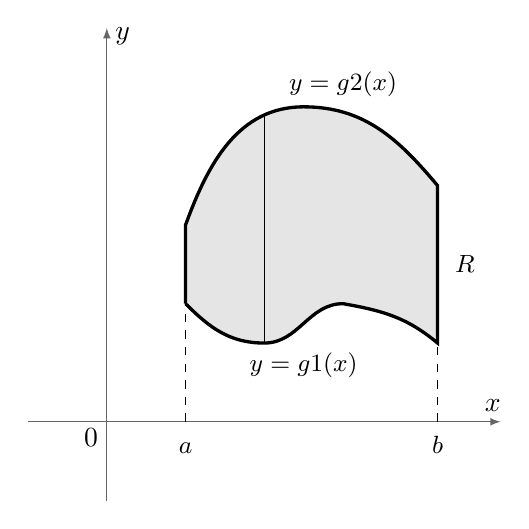
\begin{tikzpicture}[every node/.style={font=\small}]
  \usetikzlibrary{arrows}
  \draw [black!60,line width=0.3pt,-latex] (-1,0) -- (5,0);
  \draw [black!60,line width=0.3pt,-latex,anchor=base] (0,-1) -- (0,5)
   node[black,shift={(0,-0.4)}] at (1,0) {$a$}
   node[black,shift={(0,-0.4)}] at (4.2,0) {$b$};
  \pgfputat{\pgfpointxyz{4.9}{0.2}{0}}{\pgfbox[center,center]{$x$}}
  \pgfputat{\pgfpointxyz{0.2}{4.9}{0}}{\pgfbox[center,center]{$y$}}
  \pgfputat{\pgfpointxyz{-0.2}{-0.2}{0}}{\pgfbox[center,center]{$0$}}
  \filldraw [black,line width=1.2pt,fill=black!10] (1,1.5) -- (1,2.5) to[out=70,in=180] (2.5,4) to[out=0,in=130]
   (4.2,3) -- (4.2,1) to[out=140,in=-10] (3,1.5) to[out=180,in=0] (2,1) to[out=180,in=-45] (1,1.5);
  \node [above] at (3,4) {$y = \ssub{g}{2}(x)$};
  \node [below] at (2.5,1) { $y = \ssub{g}{1}(x)$};
  \node [right] at (4.3,2) {$R$};
  \draw [dashed] (1,0) -- (1,1.5);
  \draw [dashed] (4.2,0) -- (4.2,1);
  \draw (2,1) -- (2,3.9);
 \end{tikzpicture}}
 \qquad\qquad
 \subfloat[][Horizontal slice: $\int_c^d \int_{\ssub{h}{1}(y)}^{\ssub{h}{2}(y)} f(x,y)\,dx\,dy$]{
 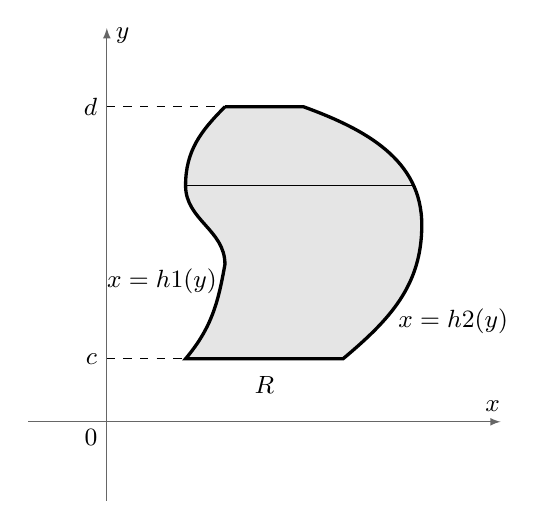
\begin{tikzpicture}
  \usetikzlibrary{arrows}
  \draw [black!60,line width=0.3pt,-latex] (-1,0) -- (5,0);
  \draw [black!60,line width=0.3pt,-latex] (0,-1) -- (0,5);
  \pgfputat{\pgfpointxyz{4.9}{0.2}{0}}{\pgfbox[center,center]{\small $x$}}
  \pgfputat{\pgfpointxyz{0.2}{4.9}{0}}{\pgfbox[center,center]{\small $y$}}
  \pgfputat{\pgfpointxyz{-0.2}{-0.2}{0}}{\pgfbox[center,center]{\small $0$}}
  \filldraw [rotate around={-90:(2.5,2.5)},black,line width=1.2pt,fill=black!10] (1,1.5) -- (1,2.5) to[out=70,in=180]
   (2.5,4) to[out=0,in=130] (4.2,3) -- (4.2,1) to[out=140,in=-10] (3,1.5) to[out=180,in=0] (2,1) to[out=180,in=-45]
   (1,1.5);
  \node [above] at (0.7,1.5) {\small $x = \ssub{h}{1}(y)$};
  \node [above] at (4.4,1) {\small $x = \ssub{h}{2}(y)$};
  \node [below] at (2,0.7) {\small $R$};
  \node [left] at (0,0.8) {\small $c$};
  \node [left] at (0,4) {\small $d$};
  \draw [dashed] (0,0.8) -- (1.1,0.8);
  \draw [dashed] (0,4) -- (1.5,4);
  \draw [rotate around={-90:(2.5,2.5)}] (2,1) -- (2,3.9);
 \end{tikzpicture}}
 \caption[]{\quad Double integral over a nonrectangular region $R$}
 \label{fig:doubleintslices}
\end{figure}

Then using the slice method from the previous section, the double integral of a real-valued function $f(x,y)$
over the region $R$, denoted by $\displaystyle\iint\limits_{R} f(x,y)\,dA$, is given by\index{$\iint$}
\begin{equation}\label{eqn:doubleintvert}
 \iint\limits_{R} f(x,y)\,dA ~=~ \int_a^b \left[ \int_{\ssub{g}{1}(x)}^{\ssub{g}{2}(x)} f(x,y)\,dy \right] \,dx
\end{equation}
This means that we take vertical slices in the region $R$ between the curves $y=\ssub{g}{1}(x)$ and $y=\ssub{g}{2}(x)$.
The symbol $dA$ is sometimes called an \emph{area element} or \emph{infinitesimal}, with the $A$ signifying area.
Note that $f(x,y)$ is first integrated with respect to $y$, with functions of $x$ as the limits of
integration. This makes sense since the result of the first iterated integral will have to be a function of $x$
alone, which then allows us to take the second iterated integral with respect to $x$.\index{area element}

Similarly, if we have a region $R$ in the $xy$-plane that is bounded on the left by a curve $x=\ssub{h}{1}(y)$,
bounded on the right by a curve $x=\ssub{h}{2}(y)$, bounded below by the horizontal line $y=c$, and bounded above by
the horizontal line $y=d$ (where $c < d$), as in Figure \ref{fig:doubleintslices}(b) (assuming that
$\ssub{h}{1}(y)$ and $\ssub{h}{2}(y)$ do not intersect on the open interval $(c,d)$), then taking horizontal slices
gives
\begin{equation}\label{eqn:doubleinthoriz}
 \iint\limits_{R} f(x,y)\,dA ~=~ \int_c^d \left[ \int_{\ssub{h}{1}(y)}^{\ssub{h}{2}(y)} f(x,y)\,dx \right] \,dy
\end{equation}

Notice that these definitions
include the case when the region $R$ is a rectangle. Also, if $f(x,y) \ge 0$ for all $(x,y)$ in the region $R$,
then $\iint\limits_{R} f(x,y)\,dA$ is the volume under the surface $z=f(x,y)$ over the region $R$.

\medskip
\hrule width \textwidth height 0.5pt
\begin{exmp}\label{exmp:doube-iterated}
Assume the region $R$ is defined by the inequalities $x^2\le y$ and $y^2\le x$.
Rewrite double integral 
 \[\iint\limits_{R} f(x,y)\,dA,\]
as an iterated integral.
\end{exmp}

\smallskip
 
\par\noindent \emph{Solution:} Let us try to write the iterated integral as in (\ref{eqn:doubleinthoriz}).

First we need to find the projection of $R$ to $y$-axis.
In other words, we need to find all $y$ such that $(x,y)$ belongs to $R$ for some $y$.
The later holds if $y^4\ge y$ or equivalently if $y\in[0,1]$; in other words $c=0$ and $d=1$.

{

\begin{wrapfigure}{r}{19 mm}
\begin{lpic}[t(0mm),b(0mm),r(0mm),l(0mm)]{pics/region-2d(1)}
\end{lpic}
\end{wrapfigure}

Now for fixed $y$, such that $0\le y\le 1$
we need to find all values $x$ such that $(x,y)$ belongs to $R$.
The later holds if $y^2\le x\ge \sqrt y$. In other words, $h_1(y)=y^2$ and $h_2(y)=\sqrt y$.
That is, 
\[\iint\limits_{R} f(x,y)\,dA
=
\int_0^1\left[
\int_{y^2}^{\sqrt{y}}f(x,y)\,dx\right]\,dy.\]

}

Note that the region $R$ does not change if you switch $x$ and $y$.
Therefore, the same integral could be written as 
\[\iint\limits_{R} f(x,y)\,dA
=
\int_0^1\,
\left[\int_{x^2}^{\sqrt{x}}f(x,y)\,dy\right]\,dx.\]


\medskip
\hrule width \textwidth height 0.5pt
\begin{exmp}\label{exmp:volplanenr}
 Find the volume $V$ under the plane $z=8x+6y$ over the plane region 
 $R$ defined by the inequalities $ 0 \le x \le 1$ and  $0 \le y \le 2x^2
 \rbrace$.
 \smallskip
 \piccaption[]{}\parpic[r]{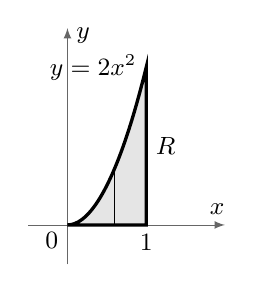
\begin{tikzpicture}
   \usetikzlibrary{arrows}
   \draw [black!60,line width=0.3pt,-latex] (-0.5,0) -- (2,0);
   \draw [black!60,line width=0.3pt,-latex] (0,-0.5) -- (0,2.5);
   \pgfputat{\pgfpointxyz{1.9}{0.2}{0}}{\pgfbox[center,center]{\small $x$}}
   \pgfputat{\pgfpointxyz{0.2}{2.4}{0}}{\pgfbox[center,center]{\small $y$}}
   \pgfputat{\pgfpointxyz{-0.2}{-0.2}{0}}{\pgfbox[center,center]{\small $0$}}
   \filldraw [black,line width=1.2pt,fill=black!10] (0,0) parabola (1,2) -- (1,0) -- (0,0);
   \node [left] at (1,2) {\small $y = 2x^2$};
   \node [right] at (1,1) {\small $R$};
   \node [below] at (1,0) {\small $1$};
   \draw (0.6,0) -- (0.6,0.72);
  \end{tikzpicture}}
 \par\noindent \emph{Solution:} The region $R$ is shown in Figure 3.2.2. Using vertical slices we get:
 \begin{align*}
  V ~&=~ \iint\limits_{R} (8x+6y)\,dA\\
   &=~ \int_0^1 \left[ \int_{0}^{2x^2} (8x+6y)\,dy \right] \,dx\\
   &=~ \int_0^1 \left( 8xy + 3y^2 \,\Big|_{y=0}^{y=2x^2} \right) \,dx\\
   &=~ \int_0^1 ( 16x^3 + 12x^4 )\,dx\\
   &=~ 4x^4 + \tfrac{12}{5}x^5 \,\Big|_0^1 ~=~ 4 + \tfrac{12}{5} ~=~ \tfrac{32}{5} ~=~ 6.4
 \end{align*}

 \piccaption[]{}\parpic[r]{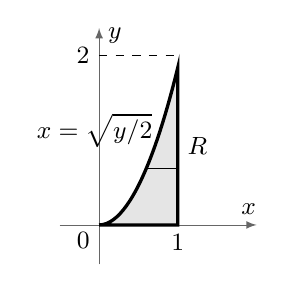
\begin{tikzpicture}
   \usetikzlibrary{arrows}
   \draw [black!60,line width=0.3pt,-latex] (-0.5,0) -- (2,0);
   \draw [black!60,line width=0.3pt,-latex] (0,-0.5) -- (0,2.5);
   \pgfputat{\pgfpointxyz{1.9}{0.2}{0}}{\pgfbox[center,center]{\small $x$}}
   \pgfputat{\pgfpointxyz{0.2}{2.4}{0}}{\pgfbox[center,center]{\small $y$}}
   \pgfputat{\pgfpointxyz{-0.2}{-0.2}{0}}{\pgfbox[center,center]{\small $0$}}
   \filldraw [black,line width=1.2pt,fill=black!10] (0,0) parabola (1,2) -- (1,0) -- (0,0);
   \node [left] at (0,2.15) {\small $2$};
   \node [left] at (0.8,1.2) {\small $x = \sqrt{y/2}$};
   \node [right] at (1,1) {\small $R$};
   \node [below] at (1,0) {\small $1$};
   \draw (0.6,0.72) -- (1,0.72);
   \draw [dashed] (0,2.15) -- (1,2.15);
  \end{tikzpicture}}
 \par\noindent We get the same answer using horizontal slices (see Figure 3.2.3):
 \begin{align*}
  V ~&=~ \iint\limits_{R} (8x+6y)\,dA\\
   &=~ \int_0^2 \left[ \int_{\sqrt{y/2}}^{1} (8x+6y)\,dx \right] \,dy\\
   &=~ \int_0^2 \left( 4x^2 + 6xy \,\Big|_{x=\sqrt{y/2}}^{x=1} \right) \,dy\\
   &=~ \int_0^2 ( 4 + 6y - (2y + \tfrac{6}{\sqrt{2}}y\sqrt{y}\,))\,dy ~=~
    \int_0^2 ( 4 + 4y - 3\sqrt{2}y^{3/2} )\,dy\\
   &=~ 4y + 2y^2 - \tfrac{6\sqrt{2}}{5}y^{5/2} \,\Big|_0^2 ~=~ 8 + 8 - \tfrac{6\sqrt{2}\sqrt{32}}{5} ~=~
    16 - \tfrac{48}{5} ~=~ \tfrac{32}{5} ~=~ 6.4
 \end{align*}
\end{exmp}
\hrule width \textwidth height 0.5pt
\begin{exmp}\label{exmp:tetra}
 Find the volume $V$ of the solid bounded by the three coordinate planes and the plane $2x+y+4z=4$.

 \begin{figure}[h]
  \centering
  \subfloat[][]{
   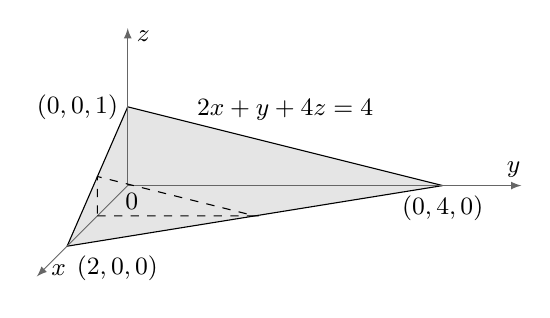
\begin{tikzpicture}
    \usetikzlibrary{arrows}
    \filldraw [black,fill=black!10] (4,0,0) -- (0,1,0) -- (0,0,2) -- (4,0,0);
    \draw [black!60,line width=0.3pt,-latex] (0,0) -- (5,0,0);
    \draw [black!60,line width=0.3pt,-latex] (0,0) -- (0,2,0);
    \draw [black!60,line width=0.3pt,-latex] (0,0) -- (0,0,3);
    \pgfputat{\pgfpointxyz{4.9}{0.2}{0}}{\pgfbox[center,center]{\small $y$}};
    \pgfputat{\pgfpointxyz{0.2}{1.9}{0}}{\pgfbox[center,center]{\small $z$}};
    \pgfputat{\pgfpointxyz{0.2}{0}{2.8}}{\pgfbox[center,center]{\small $x$}};
    \pgfputat{\pgfpointxyz{0.05}{-0.2}{0}}{\pgfbox[center,center]{\small $0$}};
    \node [below] at (4,0,0) {\small $(0,4,0)$};
    \node [left] at (0,1,0) {\small $(0,0,1)$};
    \node [below right] at (0,0,2) {\small $(2,0,0)$};
    \node [above] at (2,0.7) {\small $2x+y+4z=4$};
    \draw [dashed] (0,0,1) -- (2,0,1) -- (0,0.5,1) -- (0,0,1);
   \end{tikzpicture}}
  \qquad\qquad
  \subfloat[][]{
   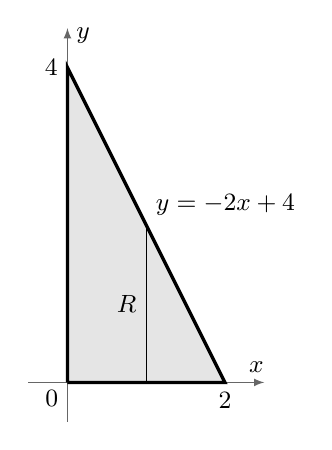
\begin{tikzpicture}
    \usetikzlibrary{arrows}
    \draw [black!60,line width=0.3pt,-latex] (-0.5,0) -- (2.5,0);
    \draw [black!60,line width=0.3pt,-latex] (0,-0.5) -- (0,4.5);
    \pgfputat{\pgfpointxyz{2.4}{0.2}{0}}{\pgfbox[center,center]{\small $x$}}
    \pgfputat{\pgfpointxyz{0.2}{4.4}{0}}{\pgfbox[center,center]{\small $y$}}
    \pgfputat{\pgfpointxyz{-0.2}{-0.2}{0}}{\pgfbox[center,center]{\small $0$}}
    \filldraw [black,line width=1.2pt,fill=black!10] (0,0) -- (0,4) -- (2,0) -- (0,0);
    \node [above right] at (1,2) {\small $y = -2x+4$};
    \node [left] at (1,1) {\small $R$};
    \node [below] at (2,0) {\small $2$};
    \node [left] at (0,4) {\small $4$};
    \draw (1,0) -- (1,2);
   \end{tikzpicture}}
  \caption[]{}
  \label{fig:volplane}
 \end{figure}

 \par\noindent \emph{Solution:} The solid is shown in Figure \ref{fig:volplane}(a) with a typical vertical slice.
 The volume $V$ is given by
 $\iint\limits_{R} f(x,y)\,dA$, where $f(x,y) = z = \frac{1}{4}(4-2x-y)$ and the region $R$, shown in Figure
 \ref{fig:volplane}(b), is $R = \lbrace (x,y): 0 \le x \le 2,~ 0 \le y \le -2x+4 \rbrace$. Using vertical
 slices in $R$ gives
 \begin{align*}
  V ~&=~ \iint\limits_{R} \tfrac{1}{4}(4-2x-y)\,dA\\
   &=~ \int_0^2 \left[ \int_{0}^{-2x+4} \tfrac{1}{4}(4-2x-y)\,dy \right] \,dx\\
   &=~ \int_0^2 \left( -\tfrac{1}{8}(4-2x-y)^2 \,\Big|_{y=0}^{y=-2x+4} \right) \,dx\\
   &=~ \int_0^2 \tfrac{1}{8}(4-2x)^2\,dx\\
   &=~ -\tfrac{1}{48}(4-2x)^3 \,\Big|_0^2 ~=~ \tfrac{64}{48} ~=~ \tfrac{4}{3}
 \end{align*}
\end{exmp}
\hrule width \textwidth height 0.5pt
\medskip

For a general region $R$, which may not be one of the types of regions we have considered so far, the double integral
$\iint\limits_{R} f(x,y)\,dA$ is defined as follows. Assume that $f(x,y)$ is a nonnegative real-valued function
and that $R$ is a bounded region in $\Real{2}$, so it
can be enclosed in some rectangle $\lbrack a,b \rbrack \times \lbrack c,d \rbrack$. 
Then divide that rectangle
into a grid of subrectangles. 
Only consider the subrectangles that are enclosed completely within the region $R$, as
shown by the shaded subrectangles in Figure \ref{fig:subrect}(a). In any such subrectangle
$\lbrack \ssub{x}{i},\ssub{x}{i+1} \rbrack \times \lbrack \ssub{y}{j},\ssub{y}{j+1} \rbrack$, pick a point
$(\ssub{x}{i*},\ssub{y}{j*})$. Then the volume under the surface $z=f(x,y)$ over that subrectangle is approximately
$f(\ssub{x}{i*},\ssub{y}{j*})\,\Delta \ssub{x}{i} \,\Delta \ssub{y}{j}$, where $\Delta \ssub{x}{i} = \ssub{x}{i+1} -
\ssub{x}{i}$, $\Delta \ssub{y}{j} = \ssub{y}{j+1} - \ssub{y}{j}$, and $f(\ssub{x}{i*},\ssub{y}{j*})$ is the height
and $\Delta \ssub{x}{i} \,\Delta \ssub{y}{j}$ is the base area of a parallelepiped, as shown in Figure
\ref{fig:subrect}(b). Then the total volume under the surface is approximately the sum of the volumes of all such
parallelepipeds, namely
\begin{equation}\label{eqn:approxvol}
 \sum_j \sum_i f(\ssub{x}{i*},\ssub{y}{j*})\,\Delta \ssub{x}{i} \,\Delta \ssub{y}{j} ~,
\end{equation}
where the summation occurs over the indices of the subrectangles inside $R$. If we take smaller and smaller
subrectangles, so that the length of the largest diagonal of the subrectangles goes to $0$, then the subrectangles
begin to fill more and more of the region $R$, and so the above sum approaches
the actual volume under the surface $z=f(x,y)$ over the region $R$. We then \emph{define}
$\iint\limits_{R} f(x,y)\,dA$ as the limit of that double summation (the limit is taken over all subdivisions of the
rectangle $\lbrack a,b \rbrack \times \lbrack c,d \rbrack$ as the largest diagonal of the subrectangles goes to $0$).

\begin{figure}[h]
 \centering
 \subfloat[][\quad Subrectangles inside the region $R$]{
  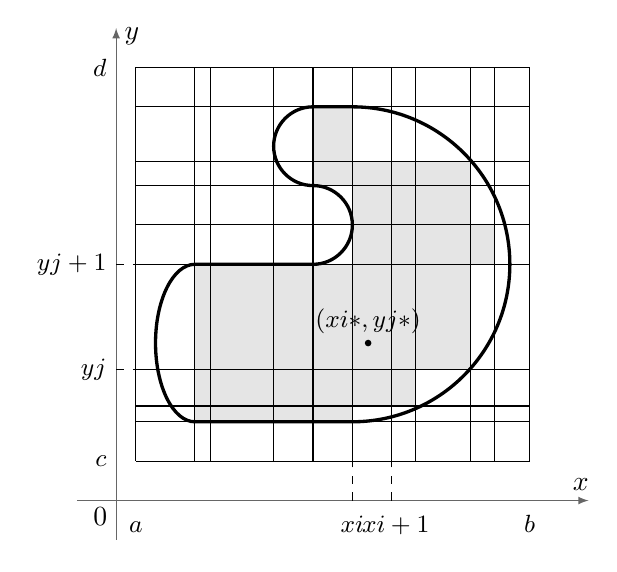
\begin{tikzpicture}[every node/.style={font=\small}]
   \usetikzlibrary{arrows}
   \draw [black!60,line width=0.3pt,-latex,anchor=base] (-0.5,0) -- (6,0)
    node[black,shift={(0,-0.4)}] at (0.25,0) {$a$}
    node[black,shift={(0,-0.4)}] at (5.25,0) {$b$}
    node[black,shift={(0,-0.4)}] at (3,0) {$\ssub{x}{i}$}
    node[black,shift={(0,-0.4)}] at (3.55,0) {$\ssub{x}{i+1}$};
   \draw [black!60,line width=0.3pt,-latex] (0,-0.5) -- (0,6);
   \pgfputat{\pgfpointxyz{5.9}{0.2}{0}}{\pgfbox[center,center]{$x$}}
   \pgfputat{\pgfpointxyz{0.2}{5.9}{0}}{\pgfbox[center,center]{$y$}}
   \pgfputat{\pgfpointxyz{-0.2}{-0.2}{0}}{\pgfbox[center,center]{$0$}}
   \fill [fill=black!10] (2.5,5) -- (2.5,4) -- (3,4) -- (3,3) -- (1,3) -- (1,1) -- (3,1) -- (3,1.2) -- (3.8,1.2) --
    (3.8,1.66) -- (4.5,1.66) -- (4.5,3) -- (4.8,3) -- (4.8,3.5) -- (4.5,3.5) -- (4.5,4.3) -- (3.8,4.3) -- (3,4.3) --
    (3,5) -- (2.5,5);
   \draw (0.25,0.5) -- (5.25,0.5) -- (5.25,5.5) -- (0.25,5.5) -- (0.25,0.5);
   \draw (0.25,1) -- (5.25,1);
   \draw (0.25,1.2) -- (5.25,1.2);
   \draw (0.25,1.66) -- (5.25,1.66);
   \draw (0.25,3) -- (5.25,3);
   \draw (0.25,3.5) -- (5.25,3.5);
   \draw (0.25,4) -- (5.25,4);
   \draw (0.25,4.3) -- (5.25,4.3);
   \draw (0.25,5) -- (5.25,5);
   \draw (1,0.5) -- (1,5.5);
   \draw (1.2,0.5) -- (1.2,5.5);
   \draw (2,0.5) -- (2,5.5);
   \draw (2.5,0.5) -- (2.5,5.5);
   \draw (3,0.5) -- (3,5.5);
   \draw (3.5,0.5) -- (3.5,5.5);
   \draw (3.8,0.5) -- (3.8,5.5);
   \draw (4.5,0.5) -- (4.5,5.5);
   \draw (4.8,0.5) -- (4.8,5.5);
   \draw [black,line width=1.2pt] (1,3) arc (90:270:0.5 and 1) -- (3,1) arc (-90:90:2 and 2) -- (2.5,5)
    arc (90:270:0.5 and 0.5) -- (2.5,4) arc (90:-90:0.5 and 0.5) -- (1,3);
   \node [left] at (0,5.5) {$d$};
   \node [left] at (0,0.5) {$c$};
   \node [left] at (0,1.66) {$\ssub{y}{j}$};
   \node [left] at (0,3) {$\ssub{y}{j+1}$};
   \draw [dashed] (3,0) -- (3,0.5);
   \draw [dashed] (3.5,0) -- (3.5,0.5);
   \draw [dashed] (0,1.66) -- (0.25,1.66);
   \draw [dashed] (0,3) -- (0.25,3);
   \fill (3.2,2) circle (1.2pt);
   \node [above] at (3.2,2) {$(\ssub{x}{i*},\ssub{y}{j*})$};
  \end{tikzpicture}}
 \qquad\qquad
 \subfloat[][\quad Parallelepiped over a subrectangle, with volume
  $f(\ssub{x}{i*},\ssub{y}{j*})\,\Delta \ssub{x}{i} \,\Delta \ssub{y}{j}$]{
  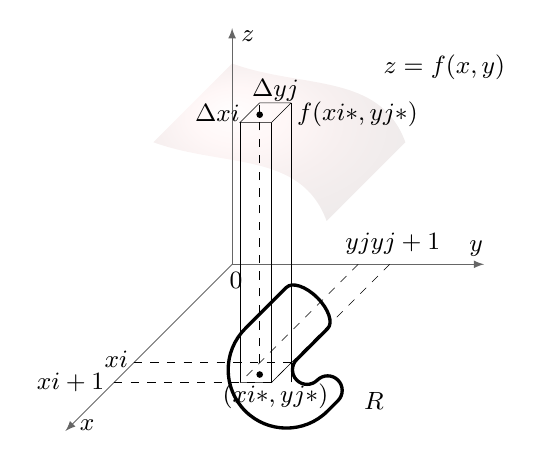
\begin{tikzpicture}
   \usetikzlibrary{arrows}
   \definecolor{planecolor}{HTML}{FFB270}
   \definecolor{surfcolor}{HTML}{006146}
   \shade [opacity=0.1,ball color=red!40] (-1,1.55) to[out=-20,in=110] (1.2,0.55) -- (2.2,1.55) to[out=110,in=-20]
    (0,2.55) -- (-1,1.55);
   \draw [black!60,line width=0.3pt,-latex] (0,0) -- (3.2,0,0);
   \draw [black!60,line width=0.3pt,-latex] (0,0) -- (0,3,0);
   \draw [black!60,line width=0.3pt,-latex] (0,0) -- (0,0,5.5);
   \pgfputat{\pgfpointxyz{3.1}{0.2}{0}}{\pgfbox[center,center]{\small $y$}};
   \pgfputat{\pgfpointxyz{0.2}{2.9}{0}}{\pgfbox[center,center]{\small $z$}};
   \pgfputat{\pgfpointxyz{0.2}{0}{5.3}}{\pgfbox[center,center]{\small $x$}};
   \pgfputat{\pgfpointxyz{0.05}{-0.2}{0}}{\pgfbox[center,center]{\small $0$}};
   \draw [scale=0.37,rotate around={-135:(0,0)},line width=1.2pt,xshift=-50pt,yshift=25pt] (1,3) arc (90:270:0.5 and 1)
    -- (3,1) arc (-90:90:2 and 2) -- (2.5,5) arc (90:270:0.5 and 0.5) -- (2.5,4) arc (90:-90:0.5 and 0.5) -- (1,3);
   \draw [dashed,line width=0.2pt] (1.6,0) -- (0.1,-1.5);
   \draw [dashed,line width=0.2pt] (2,0) -- (0.5,-1.5);
   \draw [dashed,line width=0.2pt] (-1.5,-1.5) -- (0.5,-1.5);
   \draw [dashed,line width=0.2pt] (-1.25,-1.25) -- (0.75,-1.25);
   \draw [line width=0.2pt] (0.1,-1.5) -- (0.1,1.8);
   \draw [line width=0.2pt] (0.5,-1.5) -- (0.5,1.8);
   \draw [dashed,line width=0.2pt] (0.35,-1.25) -- (0.35,2.05);
   \draw [line width=0.2pt] (0.75,-1.5) -- (0.75,2.05);
   \draw [line width=0.2pt] (0.75,2.05) -- (0.35,2.05) -- (0.1,1.8) -- (0.5,1.8) -- (0.75,2.05);
   \draw [line width=0.2pt] (0.1,-1.5) -- (0.5,-1.5) -- (0.75,-1.25);
   \node [below] at (1.8,-1.5) {\small $R$};
   \node [left] at (-1.2,-1.2) {\small $\ssub{x}{i}$};
   \node [left] at (-1.5,-1.5) {\small $\ssub{x}{i+1}$};
   \node [above] at (1.6,0) {\small $\ssub{y}{j}$};
   \node [above] at (2.2,0) {\small $\ssub{y}{j+1}$};
   \node [right] at (1.8,2.5) {\small $z = f(x,y)$};
   \node [above] at (0.55,1.95) {\small $\Delta \ssub{y}{j}$};
   \node [left] at (0.22,1.92) {\small $\Delta \ssub{x}{i}$};
   \fill (0.35,-1.4) circle (1.2pt);
   \node [below] at (0.55,-1.4) {\small $(\ssub{x}{i*},\ssub{y}{j*})$};
   \fill (0.35,1.9) circle (1.2pt);
   \node [right] at (0.7,1.9) {\small $f(\ssub{x}{i*},\ssub{y}{j*})$};
  \end{tikzpicture}}
 \caption[]{\quad Double integral over a general region $R$}
 \label{fig:subrect}
\end{figure}

A similar definition can be made for a function $f(x,y)$ that is not necessarily always nonnegative: just replace
each mention of volume by the negative volume in the description above when $f(x,y) < 0$.
In the case of a region of the type shown in Figure \ref{fig:doubleintslices}, using the definition
of the Riemann integral from single-variable calculus, our definition of $\iint\limits_{R} f(x,y)\,dA$
reduces to a sequence of two iterated integrals.

Finally, the region $R$ does not have to be\index{improper integral}\index{integral!improper}
bounded. 
We can evaluate \emph{improper} double integrals 
(that is, over an unbounded region, or over a region which
contains points where the function $f(x,y)$ is not defined) 
as a sequence of iterated improper single-variable
integrals.

\medskip
\hrule width \textwidth height 0.5pt

\begin{exmp}
 Evaluate 
 \[\int_1^{\infty}\, \int_0^{1/{x^2}} 2y \,dy\,dx.\]
\par\noindent \emph{Solution:}
 \begin{align*}
  \int_1^{\infty} \,\int_0^{1/{x^2}} 2y \,dy\,dx ~&=~
   \int_1^{\infty} \left(y^2 \,\Big|_{y=0}^{y=1/{x^2}} \right) \,dx\\
   &=~ \int_1^{\infty} x^{-4}\,dx 
   ~=~ -\tfrac{1}{3} x^{-3} \,\Big|_{1}^{\infty} ~=~ 0 - (-\tfrac{1}{3}) ~=~ \tfrac{1}{3}
 \end{align*}
\end{exmp}
\startexercises\label{sec3dot2}
\probs{A}
\par\noindent For Exercises \ref{ex:iint-start}--\ref{ex:iint-end}, evaluate the given double integral.
\begin{enumerate}[\bfseries 1.]
 \begin{multicols}{2}
  \item\label{ex:iint-start} $\displaystyle\int_0^1 \displaystyle\int_{\sqrt{x}}^1 24x^2 y \,dy\,dx$
  \item $\displaystyle\int_0^{\pi} \displaystyle\int_0^y \sin x \,dx\,dy$
 \end{multicols}
 \begin{multicols}{2}
  \item $\displaystyle\int_1^2 \displaystyle\int_0^{\ln x} 4x \,dy\,dx$
  \item $\displaystyle\int_0^2 \displaystyle\int_0^{2y} e^{y^2} \,dx\,dy$
 \end{multicols}
 \begin{multicols}{2}
  \item $\displaystyle\int_0^{\pi /2} \displaystyle\int_0^y \cos x \,\sin y \,dx\,dy$
  \item $\displaystyle\int_0^{\infty} \displaystyle\int_0^{\infty} xye^{-(x^2 + y^2 )} \,dx\,dy$
 \end{multicols}
 \begin{multicols}{2}
  \item $\displaystyle\int_0^2 \displaystyle\int_0^y 1 \,dx\,dy$
  \item\label{ex:iint-end} $\displaystyle\int_0^1 \displaystyle\int_0^{x^2} 2 \,dy\,dx$
 \end{multicols}
 \suspend{enumerate}
For Exercises \ref{ex:iint-R-start}--\ref{ex:iint-R-end} evaluate 
 \[\iint\limits_{R} f(x,y)\,dA,\]
 where
\resume{enumerate}[{[\bfseries 1.]}]
\item\label{ex:iint-R-start}  $f(x,y)=xy$ and $R$ is the intersection of the unit disc $x^2+y^2\le 1$ and the positive quadrant.
\item\label{ex:iint-R-end}  $f(x,y)=x^2+y$ and $R$ is the triangle with vertices $(0,0)$, $(2,0)$ and $(0,1)$.
 
 \item Find the volume $V$ of the solid bounded by the three coordinate planes and the plane $x+y+z=1$.
 \item Find the volume $V$ of the solid bounded by the three coordinate planes and the plane $3x+2y+5z=6$.
\suspend{enumerate}
\probs{B}
\resume{enumerate}[{[\bfseries 1.]}]
 \item Explain why the double integral $\iint\limits_{R} 1\,dA$ gives the area of the region $R$. For simplicity,
  you can assume that $R$ is a region of the type shown in Figure \ref{fig:doubleintslices}(a).
\suspend{enumerate}
\probs{C}
\resume{enumerate}[{[\bfseries 1.]}]
 \piccaption[]{}\parpic[r]{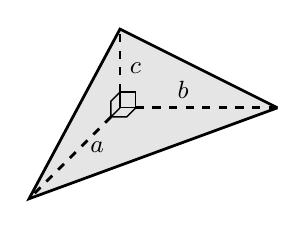
\begin{tikzpicture}
   \usetikzlibrary{arrows}
   \filldraw [black,fill=black!10,line width=1pt] (2,0,0) -- (0,1,0) -- (0,0,3) -- (2,0,0);
   \draw [dashed,line width=1pt] (0.2,0,0) -- (2,0,0);
   \draw [dashed,line width=1pt] (0,0.2,0) -- (0,1,0);
   \draw [dashed,line width=1pt] (0,0,0.3) -- (0,0,3);
   \node [above] at (0.8,0,0) {\small $b$};
   \node [right] at (0,0.5,0) {\small $c$};
   \node [right] at (0,0,1.3) {\small $a$};
   \draw [line width=0.5pt] (0,0.2,0) -- (0.2,0.2,0) -- (0.2,0,0) -- (0,0,0) -- (0,0.2,0);
   \draw [line width=0.5pt] (0,0.2,0) -- (0,0.2,0.3) -- (0,0,0.3) -- (0,0,0);
   \draw [line width=0.5pt] (0,0,0.3) -- (0.2,0,0.3) -- (0.2,0,0);
  \end{tikzpicture}}
 \item Prove that the volume of a tetrahedron with mutually perpendicular adjacent sides of lengths $a$, $b$, and $c$,
  as in Figure 3.2.6, is $\frac{abc}{6}$. (\emph{Hint: Mimic Example \ref{exmp:tetra}, and recall from Section 1.5 how
  three noncollinear points determine a plane.})
 \item Show how Exercise 12 can be used to solve Exercise 10.
\suspend{enumerate}
\probs{B}\\
For Exercises \ref{ex:iint-dom-start}--\ref{ex:iint-dom-end} rewrite double integral 
 \[\iint\limits_{R} f(x,y)\,dA,\]
 as an iterated integral. (\emph{Hint: try to visualize the region.})
\resume{enumerate}[{[\bfseries 1.]}]
\item\label{ex:iint-dom-start} If the region $R$ is defined by the inequalities $2y^2\le x\le 1+y^2$.
\item\label{ex:iint-dom-end} If the region $R$ is defined by the inequalities $x\le 2y\le 4x\le 1$.
\end{enumerate}
\newpage
%Begin Section 3.3
\section{Triple Integrals}
Our definition of a double integral of a real-valued function $f(x,y)$ over a region $R$ in $\Real{2}$ can be
extended to define a \emph{triple integral} of a real-valued function $f(x,y,z)$ over a \emph{solid} $S$ in
$\Real{3}$. We simply proceed as before: the solid $S$ can be enclosed in some rectangular parallelepiped, which is
then divided into subparallelepipeds. In each subparallelepiped inside $S$, with sides of lengths $\Delta x$,
$\Delta y$ and $\Delta z$, pick a point $(\ssub{x}{*},\ssub{y}{*},\ssub{z}{*})$. 
Then define the triple
integral of $f(x,y,z)$ over $S$, denoted by $\iiint\limits_{S} f(x,y,z)\,dV$, by\index{$\iiint$}
\begin{equation}
 \iiint\limits_{S} f(x,y,z)\,dV ~=~
  \lim \sum \sum \sum f(\ssub{x}{*},\ssub{y}{*},\ssub{z}{*})\,\Delta x\,\Delta y\,\Delta z ~,
\end{equation}
where the limit is over all divisions of the rectangular parallelepiped enclosing $S$ into subparallelepipeds whose
largest diagonal is going to $0$, and the triple summation is over all the subparallelepipeds inside $S$. It can be
shown that this limit does not depend on the choice of the rectangular parallelepiped enclosing $S$. The symbol $dV$
is often called the \emph{volume element}.\index{volume element}

Physically,\index{integral!triple}\index{triple integral}
what does the triple integral represent? We saw that a double integral could be thought of as the volume under a
two-dimensional surface. It turns out that the triple integral simply generalizes this idea: it can be thought of as
representing the \emph{hypervolume} under a three-dimensional \emph{hypersurface} $w=f(x,y,z)$ whose graph lies in
$\Real{4}$. In general, the word ``volume'' is\index{hypervolume}\index{hypersurface}
often used as a general term to signify the same concept for any $n$-dimensional object 
(including length in $\Real{1}$, area in $\Real{2}$ and volume in $\Real{3}$). 
It may be hard to get a grasp on the
concept of the ``volume'' of a four-dimensional object, but at least we now know how to calculate that volume!

In the case where $S$ is a rectangular parallelepiped
$\lbrack \ssub{x}{1},\ssub{x}{2} \rbrack \times \lbrack \ssub{y}{1},\ssub{y}{2} \rbrack \times \lbrack
\ssub{z}{1},\ssub{z}{2} \rbrack$, that is, $S = \lbrace (x,y,z): \ssub{x}{1} \le x \le \ssub{x}{2},~
\ssub{y}{1} \le y \le \ssub{y}{2},~\ssub{z}{1} \le z \le \ssub{z}{2} \rbrace$, the triple integral is a sequence
of three iterated integrals, namely
\begin{equation}
 \iiint\limits_{S} f(x,y,z)\,dV ~=~
  \int_{\ssub{z}{1}}^{\ssub{z}{2}} \int_{\ssub{y}{1}}^{\ssub{y}{2}} \int_{\ssub{x}{1}}^{\ssub{x}{2}} f(x,y,z)\,
  dx\,dy\,dz ~,
\end{equation}
where the order of integration does not matter. This is the simplest case.

A more complicated case is where $S$ is a solid which is bounded below by a surface $z=\ssub{g}{1}(x,y)$, bounded above
by a surface $z=\ssub{g}{2}(x,y)$, $y$ is bounded between two curves $\ssub{h}{1}(x)$ and $\ssub{h}{2}(x)$, and $x$
varies between $a$ and $b$. Then
\begin{equation}\label{eqn:vsolid}
 \iiint\limits_{S} f(x,y,z)\,dV 
 ~=~
 \int_{a}^{b}
 \,\, 
 \int_{\ssub{h}{1}(x)}^{\ssub{h}{2}(x)}
 \,\,
 \int_{\ssub{g}{1}(x,y)}^{\ssub{g}{2}(x,y)} f(x,y,z)\,
  dz\,dy\,dx ~.
\end{equation}
Notice in this case that the first iterated integral will result in a function of $x$ and $y$ (since its limits
of integration are functions of $x$ and $y$), which then leaves you with a double integral of a type that we learned
how to evaluate in Section 3.2. There are, of course, many variations on this case (for example, changing the roles of
the variables $x$, $y$, $z$), so as you can probably tell, triple integrals can be quite tricky. At this point, just
learning how to evaluate a triple integral, regardless of what it represents, is the most important thing. We will see
some other ways in which triple integrals are used later in the text.

\medskip
\hrule width \textwidth height 0.5pt
\begin{exmp}
 Evaluate $\displaystyle\int_0^3 \displaystyle\int_0^2 \displaystyle\int_0^1 (xy+z) \,dx\,dy\,dz$.\smallskip
 \par\noindent \emph{Solution:}
 \begin{align*}
  \int_0^3 \int_0^2 \int_0^1 (xy+z) \,dx\,dy\,dz ~&=~
   \int_0^3 \int_0^2 \left( \tfrac{1}{2}x^2 y + xz \, \Big|_{x=0}^{x=1} \right) \,dy\,dz\\
   &=~ \int_0^3 \int_0^2 \left( \tfrac{1}{2}y + z \right) \,dy\,dz\\
   &=~ \int_0^3 \left( \tfrac{1}{4}y^2 + yz \,\Big|_{y=0}^{y=2} \right) \,dz\\
   &=~ \int_0^3 (1+2z) \,dz\\
   &=~ z + z^2 \,\Big|_0^3 ~=~ 12
 \end{align*}
\end{exmp}
\hrule width \textwidth height 0.5pt
\begin{exmp}
 Evaluate 
 \[\int_0^1\,\, \int_0^{1-x}\,\, \int_0^{2-x-y} (x+y+z)\,dz\,dy\,dx.\]
 \par\noindent \emph{Solution:}
 \begin{align*}
  \int_0^1\,\, \int_0^{1-x}\,\, \int_0^{2-x-y} (x+y+z) \,dz\,dy\,dx ~&=~
   \int_0^1 \int_0^{1-x} \left( (x+y)z+ \tfrac{1}{2}z^2 \, \Big|_{z=0}^{z=2-x-y} \right) \,dy\,dx\\
   &=~ \int_0^1 \int_0^{1-x} \left( (x+y)(2-x-y) + \tfrac{1}{2}(2-x-y)^2 \right) \,dy\,dx\\
   &=~ \int_0^1 \int_0^{1-x} \left( 2 - \tfrac{1}{2}x^2 - xy - \tfrac{1}{2}y^2 \right) \,dy\,dx\\
   &=~ \int_0^1 \left( 2y-\tfrac{1}{2}x^2 y -xy- \tfrac{1}{2}xy^2 - \tfrac{1}{6}y^3 \,\Big|_{y=0}^{y=1-x} \right) \,dx\\
   &=~ \int_0^1 \left( \tfrac{11}{6} - 2x + \tfrac{1}{6}x^3 \right) \,dx\\
   &=~ \tfrac{11}{6}x - x^2 + \tfrac{1}{24}x^4 \,\Big|_0^1 ~=~ \tfrac{7}{8}
 \end{align*}
\end{exmp}
\hrule width \textwidth height 0.5pt
\smallskip
Note that the volume $V$ of a solid in $\Real{3}$ is given by
\begin{equation}
 V ~=~ \iiint\limits_{S} 1\,dV ~.
\end{equation}
Since the function being integrated is the constant $1$, then the above triple integral reduces to a double integral of
the types that we considered in the previous section if the solid is bounded above by some surface $z=f(x,y)$ and
bounded below by the $xy$-plane $z=0$. There are many other possibilities. For example, the solid could be bounded
below and above by surfaces $z=\ssub{g}{1}(x,y)$ and $z=\ssub{g}{2}(x,y)$, respectively, with $y$ bounded between
two curves $\ssub{h}{1}(x)$ and $\ssub{h}{2}(x)$, and $x$ varies between $a$ and $b$. Then
\begin{displaymath}
 V = \iiint\limits_{S} 1\,dV =
  \int_{a}^{b}\,\, 
  \int_{\ssub{h}{1}(x)}^{\ssub{h}{2}(x)}\,\, 
  \int_{\ssub{g}{1}(x,y)}^{\ssub{g}{2}(x,y)} 1\,dz\,dy\,dx 
  =
  \int_{a}^{b}\,\, 
  \int_{\ssub{h}{1}(x)}^{\ssub{h}{2}(x)} 
  \left( \ssub{g}{2}(x,y) - \ssub{g}{1}(x,y) \right) \,dy\,dx
\end{displaymath}
just like in equation (\ref{eqn:vsolid}). See Exercise 10 for an example.
\startexercises\label{sec3dot3}
\probs{A}
\par\noindent For Exercises 1--8, evaluate the given triple integral.
\begin{enumerate}[\bfseries 1.]
 \begin{multicols}{2}
  \item $\displaystyle\int_0^3 \displaystyle\int_0^2 \displaystyle\int_0^1 xyz \,dx\,dy\,dz$
  \item $\displaystyle\int_0^1 \displaystyle\int_0^x \displaystyle\int_0^y xyz \,dz\,dy\,dx$
 \end{multicols}
 \begin{multicols}{2}
  \item $\displaystyle\int_0^{\pi} \displaystyle\int_0^x \displaystyle\int_0^{xy} x^2 \sin z \,dz\,dy\,dx$
  \item $\displaystyle\int_0^1 \displaystyle\int_0^z \displaystyle\int_0^y ze^{y^2} \,dx\,dy\,dz$
 \end{multicols}
 \begin{multicols}{2}
  \item $\displaystyle\int_1^e \displaystyle\int_0^y \displaystyle\int_0^{1/y} x^2 z \,dx\,dz\,dy$
  \item $\displaystyle\int_1^2 \displaystyle\int_0^{y^2} \displaystyle\int_0^{z^2} yz \,dx\,dz\,dy$
 \end{multicols}
 \begin{multicols}{2}
  \item $\displaystyle\int_1^2 \,\,\displaystyle\int_2^4\,\, \displaystyle\int_0^3 1 \,dx\,dy\,dz$
  \item $\displaystyle\int_0^1\,\, \displaystyle\int_0^{1-x}\,\, \displaystyle\int_0^{1-x-y} 1 \,dz\,dy\,dx$
 \end{multicols}
 \item Let $M$ be a constant. 
 Show that 
 \[\int_{\ssub{z}{1}}^{\ssub{z}{2}}
 \,\int_{\ssub{y}{1}}^{\ssub{y}{2}}
 \,\int_{\ssub{x}{1}}^{\ssub{x}{2}} 
 M\,dx\,dy\,dz 
 = 
 M(\ssub{z}{2} - \ssub{z}{1})(\ssub{y}{2} - \ssub{y}{1})
  (\ssub{x}{2} - \ssub{x}{1}).\]
\suspend{enumerate}
\probs{B}
\resume{enumerate}[{[\bfseries 1.]}]
 \item Find the volume $V$ of the solid $S$ bounded by the three coordinate planes, bounded above by the plane
  $x+y+z=2$, and bounded below by the plane $z=x+y$.
\suspend{enumerate}
\probs{C}
\resume{enumerate}[{[\bfseries 1.]}]
 \item Show that 
 \[\displaystyle\int_a^b \displaystyle\int_a^z \displaystyle\int_a^y f(x)\,dx\,dy\,dz =
  \displaystyle\int_a^b \tfrac{(b-x)^2 }{2} f(x)\,dx.\] 
  (\emph{Hint: Think of how changing the order of integration in
  the triple integral changes the limits of integration.})
\end{enumerate}
\newpage
%Begin Section 3.4
\section{Numerical Approximation of Multiple Integrals}
\label{sec:Numerical Approximation of Multiple Integrals}
As you have seen, calculating multiple integrals is tricky even for simple functions and regions. For complicated
functions, it may not be possible to evaluate one of the iterated integrals in a simple closed form. Luckily there
are numerical methods for approximating the value of a multiple integral. The method we will discuss is called the
\emph{Monte Carlo method}. The idea behind it is based on the concept of the \emph{average value} of a function, which
you learned in single-variable calculus. Recall that for a continuous function $f(x)$, the \textbf{average value}
$\bar{f}$ of $f$ over an interval $\lbrack a,b \rbrack$ is defined
as\index{Monte Carlo method}\index{average value}
\begin{equation}\label{eqn:favg}
 \bar{f} ~=~ \frac{1}{b-a}\int_a^b f(x)\,dx ~.
\end{equation}

The quantity $b-a$ is the length of the interval $\lbrack a,b \rbrack$, which can be thought of as the ``volume'' of
the interval. Applying the same reasoning to functions of two or three variables, we define the \textbf{average
value} of $f(x,y)$ over a region $R$ to be
\begin{equation}\label{eqn:favg2}
 \bar{f} ~=~ \frac{1}{A(R)}\iint\limits_{R} f(x,y)\,dA ~,
\end{equation}
where $A(R)$ is the area of the region $R$, and we define the \textbf{average
value} of $f(x,y,z)$ over a solid $S$ to be
\begin{equation}\label{eqn:favg3}
 \bar{f} ~=~ \frac{1}{V(S)}\iiint\limits_{S} f(x,y,z)\,dV ~,
\end{equation}
where $V(S)$ is the volume of the solid $S$. Thus, for example, we have
\begin{equation}\label{eqn:favgint2}
 \iint\limits_{R} f(x,y)\,dA ~=~ A(R)\bar{f} ~.
\end{equation}
The average value of $f(x,y)$ over $R$ can be thought of as representing the sum of all the values of $f$ divided by the number of points in $R$. 
However, we can not take the sum literary since there are an infinite number of points in any region (in fact, uncounably many --- one can not enumerate them by natural numbers). 
But what if we took a very large number $N$ of \emph{random} points in the region $R$ (which can be generated by a computer) and then took the
average of the values of $f$ for those points, and used that
average as the value of $\bar{f}$? This is exactly what the Monte Carlo method does. So in formula (\ref{eqn:favgint2})
the approximation we get is
\begin{equation}\label{eqn:monte}
 \iint\limits_{R} f(x,y)\,dA ~\approx~ A(R)\bar{f} \pm A(R)\sqrt{\frac{\overline{f^2} - (\bar{f})^2}{N}} ~,
\end{equation}
where
\begin{equation}
 \bar{f} ~=~ \frac{1}{N}\sum_{i=1}^N f(\ssub{x}{i},\ssub{y}{i}) \quad \text{and} \quad \overline{f^2} ~=~
 \frac{1}{N} \sum_{i=1}^N (f(\ssub{x}{i},\ssub{y}{i}))^2~,
\end{equation}
with the sums taken over the $N$ random points $(\ssub{x}{1},\ssub{y}{1})$, $\ldots$, $(\ssub{x}{N},\ssub{y}{N})$.
The $\pm$ ``error term'' in formula (\ref{eqn:monte}) does not really provide
hard bounds on the approximation. It represents a single \emph{standard deviation} from the \emph{expected} value of the
integral. That is, it provides a \emph{likely} bound on the error. Due to its use of random points, the Monte Carlo
method is an example of a \emph{probabilistic} method (as opposed to \emph{deterministic} methods such as Newton's
method, which use a specific formula for generating points).

For example, we can use formula (\ref{eqn:monte}) to approximate the volume $V$ under the plane $z=8x+6y$ over the
rectangle $R = \lbrack 0,1 \rbrack \times \lbrack 0,2 \rbrack$. In Example \ref{exmp:volplane} in Section 3.1, we showed
that the actual volume is $20$. Below is a code listing (montecarlo.java) for a Java program that calculates the volume,
using a number of points $N$ that is passed on the command line as a parameter.

\medskip
\definecolor{codecolor}{HTML}{FFF7E0}
\lstset{language=Java,showstringspaces=false,
basicstyle={\small\fontfamily{fvm}\fontseries{m}\selectfont},
columns=fullflexible,backgroundcolor=\color{codecolor},
commentstyle={\color{blue}\small\fontfamily{fvm}\itshape\selectfont},
keywordstyle={\small\fontfamily{fvm}\fontseries{b}\selectfont},keepspaces=true,
float=h,caption={\hspace{1em}Program listing for montecarlo.java},label=montejava,stringstyle=\color{red},
frame=single,aboveskip=\medskipamount,belowskip=\medskipamount,captionpos=b}
\begin{lstlisting}
//Program to approximate the double integral of f(x,y)=8x+6y
//over the rectangle [0,1]x[0,2].
public class montecarlo {
 public static void main(String[] args) {
   //Get the number N of random points as a command-line parameter
   int N = Integer.parseInt(args[0]);
   double x = 0; //x-coordinate of a random point
   double y = 0; //y-coordinate of a random point
   double f = 0.0; //Value of f at a random point
   double mf = 0.0; //Mean of the values of f
   double mf2 = 0.0; //Mean of the values of f^2
   for (int i=0;i<N;i++) { //Get the random coordinates
      x = Math.random(); //x is between 0 and 1
      y = 2 * Math.random(); //y is between 0 and 2
      f = 8*x + 6*y; //Value of the function
      mf = mf + f; //Add to the sum of the f values
      mf2 = mf2 + f*f; //Add to the sum of the f^2 values
   }
   mf = mf/N; //Compute the mean of the f values
   mf2 = mf2/N; //Compute the mean of the f^2 values
   System.out.println("N = " + N + ": integral = " + vol()*mf + " +/- "
    + vol()*Math.sqrt((mf2 - Math.pow(mf,2))/N)); //Print the result
 }
 //The volume of the rectangle [0,1]x[0,2]
 public static double vol() {
   return 1*2;
 }
}
\end{lstlisting}
\medskip

The results of running this program with various numbers of random points 
(for instance, \texttt{java montecarlo 100}) 
are shown below:

\begin{verbatim}
N = 10:      19.36543087722646  +/- 2.7346060413546147
N = 100:     21.334419561385353 +/- 0.7547037194998519
N = 1000:    19.807662237526227 +/- 0.26701709691370235
N = 10000:   20.080975812043256 +/- 0.08378816229769506
N = 100000:  20.009403854556716 +/- 0.026346782289498317
N = 1000000: 20.000866994982314 +/- 0.008321168748642816
\end{verbatim}

As you can see, the approximation is fairly good.
As $N \to \infty$, it can be shown that the Monte Carlo approximation converges to the actual volume
(on the order of $O(\sqrt{N})$, in computational complexity terminology).

In the above example the region $R$ was a rectangle. To use the Monte Carlo method for a nonrectangular
(bounded) region $R$, only a slight modification is needed. Pick a rectangle $\tilde{R}$ that encloses $R$, and
generate
random points in that rectangle as before. Then use those points in the calculation of $\bar{f}$ only if they are inside
$R$. There is no need to calculate the area of $R$ for formula (\ref{eqn:monte}) in this case, since the exclusion of
points not inside $R$ allows you to use the area of the rectangle $\tilde{R}$ instead, similar to before.

For instance, in
Example \ref{exmp:volplanenr} we showed that the volume under the surface $z=8x+6y$ over the
nonrectangular region $R = \lbrace (x,y): 0 \le x \le 1,~ 0 \le y \le 2x^2 \rbrace$ is $6.4$. Since the rectangle
$\tilde{R} = \lbrack 0,1 \rbrack \times \lbrack 0,2 \rbrack$ contains $R$, we can use the same
program as before, with the only change being a check to see if $y < 2x^2$
for a random point $(x,y)$ in $\lbrack 0,1 \rbrack \times \lbrack 0,2 \rbrack$. Listing
\ref{montejava2} below contains the code (montecarlo2.java):

\medskip
\definecolor{codecolor}{HTML}{FFF7E0}
\lstset{language=Java,showstringspaces=false,
basicstyle={\small\fontfamily{fvm}\fontseries{m}\selectfont},
columns=fullflexible,backgroundcolor=\color{codecolor},
commentstyle={\color{blue}\small\fontfamily{fvm}\itshape\selectfont},
keywordstyle={\small\fontfamily{fvm}\fontseries{b}\selectfont},keepspaces=true,
float=h,caption={\hspace{1em}Program listing for montecarlo2.java},label=montejava2,stringstyle=\color{red},
frame=single,aboveskip=\medskipamount,belowskip=\medskipamount,captionpos=b}
\begin{lstlisting}
//Program to approximate the double integral of f(x,y)=8x+6y over the
//region bounded by x=0, x=1, y=0, and y=2x^2
public class montecarlo2 {
 public static void main(String[] args) {
   //Get the number N of random points as a command-line parameter
   int N = Integer.parseInt(args[0]);
   double x = 0; //x-coordinate of a random point
   double y = 0; //y-coordinate of a random point
   double f = 0.0; //Value of f at a random point
   double mf = 0.0; //Mean of the values of f
   double mf2 = 0.0; //Mean of the values of f^2
   for (int i=0;i<N;i++) { //Get the random coordinates
      x = Math.random(); //x is between 0 and 1
      y = 2 * Math.random(); //y is between 0 and 2
      if (y < 2*Math.pow(x,2)) { //The point is in the region
         f = 8*x + 6*y; //Value of the function
         mf = mf + f; //Add to the sum of the f values
         mf2 = mf2 + f*f; //Add to the sum of the f^2 values
      }
   }
   mf = mf/N; //Compute the mean of the f values
   mf2 = mf2/N; //Compute the mean of the f^2 values
   System.out.println("N = " + N + ": integral = " + vol()*mf +
    " +/- " + vol()*Math.sqrt((mf2 - Math.pow(mf,2))/N));
 }
 //The volume of the rectangle [0,1]x[0,2]
 public static double vol() {
   return 1*2;
 }
}
\end{lstlisting}

The results of running the program with various numbers of random points (for instance, \texttt{java montecarlo2 1000})
are shown below:

\begin{verbatim}
N = 10:      integral = 6.95747529014894 +/- 2.9185131565120592
N = 100:     integral = 6.3149056229650355 +/- 0.9549009662159909
N = 1000:    integral = 6.477032813858756 +/- 0.31916837260973624
N = 10000:   integral = 6.349975080015089 +/- 0.10040086346895105
N = 100000:  integral = 6.440184132811864 +/- 0.03200476870881392
N = 1000000: integral = 6.417050897922222 +/- 0.01009454409789472
\end{verbatim}

To use the Monte Carlo method to evaluate triple integrals, you will need to generate random triples $(x,y,z)$ in a
parallelepiped, instead of random pairs $(x,y)$ in a rectangle, and use the volume of the parallelepiped instead of the
area of a rectangle in formula (\ref{eqn:monte}) (see Exercise 2). For a more detailed discussion of numerical
integration methods, see \cite{ptvf} et al.
\startexercises\label{sec3dot4}
\probs{C}
\begin{enumerate}[\bfseries 1.]
 \item Write a program that uses the Monte Carlo method to approximate the double integral
  \[\iint\limits_{R} e^{xy}\,dA,\] 
  where $R = \lbrack 0,1 \rbrack \times \lbrack 0,1 \rbrack$. Show the program output
  for $N=10$, $100$, $1000$, $10000$, $100000$ and $1000000$ random points.
 \item Write a program that uses the Monte Carlo method to approximate the triple integral
  \[\iiint\limits_{S} e^{xyz}\,dV,\] 
  where $S= \lbrack 0,1 \rbrack \times \lbrack 0,1 \rbrack \times \lbrack 0,1 \rbrack$.
  Show the program output for $N=10$, $100$, $1000$, $10000$, $100000$ and $1000000$ random points.
 \item Repeat Exercise 1 with the region $R = \lbrace (x,y): -1 \le x \le 1,~ 0 \le y \le x^2 \rbrace$.
 \item Repeat Exercise 2 with the solid $S = \lbrace (x,y,z): 0 \le x \le 1,~ 0 \le y \le 1,~
  0 \le z \le 1 - x - y \rbrace$.
 \item Use the Monte Carlo method to approximate the volume of a sphere of radius $1$.
 \item Use the Monte Carlo method to approximate the volume of the ellipsoid $\frac{x^2}{9}+\frac{y^2}{4}+
  \frac{z^2}{1}=1$.
\end{enumerate}
\newpage
%Begin Section 3.5
\section{Change of Variables in Multiple Integrals}
Given the difficulty of evaluating multiple integrals, the reader may be wondering if it is possible to simplify
those integrals using a suitable substitution for the variables. The answer is yes, though it is a bit more complicated
than the substitution method which you learned in single-variable calculus.\index{change of variable}

Recall that if you are given, for example, the definite integral
\begin{displaymath}
 \int_1^2 x^3 \sqrt{x^2 - 1}\,dx ~,
\end{displaymath}
then you would make the substitution
\begin{align*}
u &= x^2 - 1 ~\Rightarrow~ x^2 = u + 1\\
du &= 2x\,dx\\
\intertext{which changes the limits of integration}
x &= 1 ~\Rightarrow~ u = 0\\
x &= 2 ~\Rightarrow~ u = 3
\end{align*}
so that we get
\begin{align*}
 \int_1^2 x^3 \sqrt{x^2 - 1}\,dx ~&=~ \int_1^2 \tfrac{1}{2}x^2 \cdot 2x \sqrt{x^2 - 1}\,dx\\
 &=~ \int_0^3 \tfrac{1}{2}(u+1)\sqrt{u}\,du\\
 &=~ \tfrac{1}{2} \int_0^3 \left( u^{3/2} + u^{1/2} \right)\,du ~~,~\text{which can be integrated to give}\\
 &=~ \tfrac{14\sqrt{3}}{5} ~.
\end{align*}
Let us take a different look at what happened when we did that substitution, which will give some motivation for how
substitution works in multiple integrals. First, we let $u = x^2 - 1$. On the interval of integration
$\lbrack 1,2 \rbrack$, the function $x \mapsto x^2 - 1$ is strictly increasing (and maps $\lbrack 1,2 \rbrack$ onto
$\lbrack 0,3 \rbrack$) and hence has an inverse function (defined on the interval $\lbrack 0,3 \rbrack$). That
is, on $\lbrack 0,3 \rbrack$ we can define $x$ as a function of $u$, namely
\begin{displaymath}
 x ~=~ g(u) ~=~ \sqrt{u+1} ~.
\end{displaymath}
Then substituting that expression for $x$ into the function $f(x) = x^3 \sqrt{x^2 - 1}$ gives
\begin{displaymath}
 f(x) ~=~ f(g(u)) ~=~ (u+1)^{3/2} \sqrt{u} ~,
\end{displaymath}
and we see that
\begin{align*}
 \frac{dx}{du} ~=~ g\,'(u) ~\Rightarrow~ dx ~&=~ g\,'(u)\,du\\
 dx ~&=~ \tfrac{1}{2} (u+1)^{-1/2}\,du ~,
\end{align*}
so since
\begin{align*}
 g(0) = 1 ~\Rightarrow~ 0 = g^{-1} (1)\\
 g(3) = 2 ~\Rightarrow~ 3 = g^{-1} (2)\\
\end{align*}
then performing the substitution as we did earlier gives
\begin{align*}
 \int_1^2 f(x)\,dx ~&=~ \int_1^2 x^3 \sqrt{x^2 - 1}\,dx\\
 &=~ \int_0^3 \tfrac{1}{2}(u+1)\sqrt{u}\,du ~~,~\text{which can be written as}\\
 &=~ \int_0^3 (u+1)^{3/2} \sqrt{u} \, \cdot \tfrac{1}{2} (u+1)^{-1/2}\,du ~~,~\text{which means}\\
 \int_1^2 f(x)\,dx ~&=~ \int_{g^{-1}(1)}^{g^{-1}(2)} f(g(u))\,g\,'(u)\,du ~.
\end{align*}

In general, if $x = g(u)$ is a one-to-one, differentiable function from an interval $\lbrack c,d \rbrack$ (which you can
think of as being on the ``$u$-axis'') onto an interval $\lbrack a,b \rbrack$ (on the $x$-axis), which means that
$g\,'(u) \ne 0$ on the interval $(c,d)$, so that $a=g(c)$ and $b=g(d)$, then $c=g^{-1}(a)$ and $d=g^{-1}(b)$, and
\begin{equation}
 \int_a^b f(x)\,dx ~=~ \int_{g^{-1}(a)}^{g^{-1}(b)} f(g(u))\,g\,'(u)\,du ~.
\end{equation}
This is called the \emph{change of variable} formula for integrals of single-variable functions, and it is what you were
implicitly using when doing integration by substitution.

This formula turns out to be a special case of a more general
formula which can be used to evaluate multiple integrals. We will state the formulas for double and triple integrals
involving real-valued functions of two and three variables, respectively.
We will assume that all the functions involved are continuously differentiable and that the regions and solids involved
all have ``reasonable'' boundaries. 
The proof of the following theorem is beyond the scope of the text.%
\footnote{See \cite[\S\,15.32 and \S\,15.62]{tm} for all the details.}

\statethm{thm:changevarint}{\index{change of variable}
 {\textbf{Change of Variables Formula for Multiple Integrals}\\
  Let $x=x(u,v)$ and $y=y(u,v)$ define a one-to-one mapping of a region $R'$ in the $uv$-plane onto a region $R$
  in the $xy$-plane such that the determinant
  \begin{equation}\label{eqn:jacob2}
   J(u,v) ~=~
    \begin{vmatrix}
     \dfrac{\partial x}{\partial u} & \dfrac{\partial x}{\partial v}\smallskip\\
     \dfrac{\partial y}{\partial u} & \dfrac{\partial y}{\partial v}
    \end{vmatrix}
  \end{equation}
  is never $0$ in $R'$. Then
  \begin{equation}\label{eqn:changevarint2}
   \iint\limits_{R} f(x,y)\,dA(x,y) ~=~ \iint\limits_{R'} f(x(u,v),y(u,v))\,\abs{J(u,v)}\,dA(u,v) ~.
  \end{equation}
  We use the notation $dA(x,y)$ and $dA(u,v)$ to denote the area element in the $(x,y)$ and $(u,v)$ coordinates,
  respectively.
  
  Similarly, if $x=x(u,v,w)$, $y=y(u,v,w)$ and $z=z(u,v,w)$ define a one-to-one mapping of a solid $S'$ in
  $uvw$-space onto a solid $S$ in $xyz$-space such that the determinant
  \begin{equation}\label{eqn:jacob3}
   J(u,v,w) ~=~
    \begin{vmatrix}
     \dfrac{\partial x}{\partial u} & \dfrac{\partial x}{\partial v} & \dfrac{\partial x}{\partial w}\smallskip\\
     \dfrac{\partial y}{\partial u} & \dfrac{\partial y}{\partial v} & \dfrac{\partial y}{\partial w}\smallskip\\
     \dfrac{\partial z}{\partial u} & \dfrac{\partial z}{\partial v} & \dfrac{\partial z}{\partial w}
    \end{vmatrix}
  \end{equation}
  is never $0$ in $S'$, then
  \begin{equation}\label{eqn:changevarint3}
   \iiint\limits_{S} f(x,y,z)\,dV(x,y,z) = \iiint\limits_{S'} f(x(u,v,w),y(u,v,w),z(u,v,w))\,\abs{J(u,v,w)}\,dV(u,v,w)~.
  \end{equation}}
}

The determinant $J(u,v)$ in formula (\ref{eqn:jacob2}) is called the \textbf{Jacobian} of $x$ and $y$ with respect to $u$
and $v$, and is sometimes written as\index{Jacobian}
\begin{equation}
 J(u,v) ~=~ \frac{\partial (x,y)}{\partial (u,v)} ~.
\end{equation}
Similarly, the Jacobian $J(u,v,w)$ of three variables is sometimes written as
\begin{equation}
 J(u,v,w) ~=~ \frac{\partial (x,y,z)}{\partial (u,v,w)} ~.
\end{equation}
Notice that formula (\ref{eqn:changevarint2}) is saying that $dA(x,y) = \abs{J(u,v)}\,dA(u,v)$, which you can think of as
a two-variable version of the relation $dx = g\,'(u)\,du$ in the single-variable case.

The following example shows how the change of variables formula is
used.\index{$\dfrac{\partial (x,y,z)}{\partial (u,v,w)}$}

\begin{exmp}
 Evaluate $\displaystyle\iint\limits_{R} e^{\frac{x-y}{x+y}} \,dA$, where $R= \lbrace (x,y): x \ge 0, y \ge 0,
 x + y \le 1 \rbrace$.\smallskip
 \par\noindent \emph{Solution:} First, note that evaluating this double integral \emph{without} using substitution is
 probably impossible, at least in a closed form. By looking at the numerator and denominator of the exponent of $e$,
 we will try the substitution $u=x-y$ and $v=x+y$. To use the change of variables formula (\ref{eqn:changevarint2}), we
 need to write both $x$ and $y$ in terms of $u$ and $v$. So solving for $x$ and $y$ gives $x=\frac{1}{2}(u+v)$ and
 $y=\frac{1}{2}(v-u)$. In Figure \ref{fig:exyint} below, we see how the mapping $x=x(u,v)=\frac{1}{2}(u+v)$,
 $y=y(u,v)=\frac{1}{2}(v-u)$ maps the region $R'$ onto $R$ in a one-to-one manner.
 
\begin{figure}[h]
 \begin{center}
  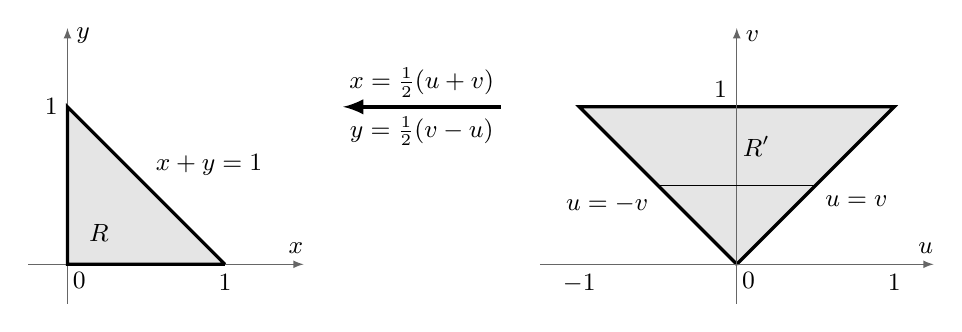
\begin{tikzpicture}
   \usetikzlibrary{arrows}
   \draw [black!60,line width=0.3pt,-latex] (-0.5,0) -- (3,0,0);
   \draw [black!60,line width=0.3pt,-latex] (0,-0.5) -- (0,3,0);
   \pgfputat{\pgfpointxyz{2.9}{0.2}{0}}{\pgfbox[center,center]{\small $x$}};
   \pgfputat{\pgfpointxyz{0.2}{2.9}{0}}{\pgfbox[center,center]{\small $y$}};
   \pgfputat{\pgfpointxyz{0.15}{-0.2}{0}}{\pgfbox[center,center]{\small $0$}};
   \filldraw [black,line width=1.2pt,fill=black!10] (2,0) -- (0,2) -- (0,0) -- (2,0);
   \node [above right] at (1,1) {\small $x+y=1$};
   \node [left] at (0,2) {\small $1$};
   \node [below] at (2,0) {\small $1$};
   \node at (0.4,0.4) {\small $R$};
   \filldraw [black,line width=1.2pt,fill=black!10] (8.5,0) -- (10.5,2) -- (6.5,2) -- (8.5,0);
   \draw [black!60,line width=0.3pt,-latex] (6,0) -- (11,0,0);
   \draw [black!60,line width=0.3pt,-latex] (8.5,-0.5) -- (8.5,3,0);
   \pgfputat{\pgfpointxyz{10.9}{0.2}{0}}{\pgfbox[center,center]{\small $u$}};
   \pgfputat{\pgfpointxyz{8.7}{2.9}{0}}{\pgfbox[center,center]{\small $v$}};
   \pgfputat{\pgfpointxyz{8.65}{-0.2}{0}}{\pgfbox[center,center]{\small $0$}};
   \draw (7.5,1) -- (9.5,1);
   \node [above left] at (8.5,2) {\small $1$};
   \node [below] at (6.5,0) {\small $-1$};
   \node [below] at (10.5,0) {\small $1$};
   \node at (8.75,1.5) {\small $R'$};
   \node [below right] at (9.5,1) {\small $u=v$};
   \node [below left] at (7.5,1) {\small $u=-v$};
   \draw [line width=1.5pt,-latex] (5.5,2) -- (3.5,2);
   \node [above] at (4.5,2) {\small $x=\frac{1}{2}(u+v)$};
   \node [below] at (4.5,2) {\small $y=\frac{1}{2}(v-u)$};
  \end{tikzpicture}
 \end{center}
 \caption[]{\quad The regions $R$ and $R'$}
 \label{fig:exyint}
\end{figure}

 Now we see that
 \begin{displaymath}
  J(u,v) ~=~
   \begin{vmatrix}
    \dfrac{\partial x}{\partial u} & \dfrac{\partial x}{\partial v}\smallskip\\
    \dfrac{\partial y}{\partial u} & \dfrac{\partial y}{\partial v}
   \end{vmatrix} ~=~
   \left| \begin{array}{rr}
    \tfrac{1}{2} & \tfrac{1}{2}\smallskip\\
    -\tfrac{1}{2} & \tfrac{1}{2}
   \end{array}\right| ~=~ \frac{1}{2} ~\Rightarrow~ \abs{J(u,v)} ~=~ \left| \frac{1}{2} \right| ~=~ \frac{1}{2} ~,
 \end{displaymath}
 so using horizontal slices in $R'$, we have
 \begin{align*}
  \iint\limits_{R} e^{\frac{x-y}{x+y}} \,dA ~&=~ \iint\limits_{R'} f(x(u,v),y(u,v))\,\abs{J(u,v)}\,dA\\
  &=~ \int_0^1 \int_{-v}^v e^{\frac{u}{v}} \, \tfrac{1}{2}\,du\,dv\\
  &=~ \int_0^1 \left( \tfrac{v}{2} e^{\frac{u}{v}} \,\Big|_{u=-v}^{u=v} \right) \,dv\\
  &=~ \int_0^1 \tfrac{v}{2} (e - e^{-1})\,dv\\
  &=~ \frac{v^2}{4} (e - e^{-1}) \,\Big|_{0}^{1} ~=~ \frac{1}{4} \left( e - \frac{1}{e} \right) ~=~ \frac{e^2 - 1}{4e}
 \end{align*}
\end{exmp}
\hrule width \textwidth height 0.5pt

\medskip

The change of variables formula can be used to evaluate double integrals in polar coordinates. Letting
\begin{displaymath}
 x ~=~ x(r,\theta) ~=~ r\cos \theta \quad \text{and} \quad y ~=~ y(r,\theta) ~=~ r\sin \theta ~,
\end{displaymath}
we have
\begin{displaymath}
 J(u,v) ~=~
  \begin{vmatrix}
   \dfrac{\partial x}{\partial r} & \dfrac{\partial x}{\partial \theta}\smallskip\\
   \dfrac{\partial y}{\partial r} & \dfrac{\partial y}{\partial \theta}
  \end{vmatrix} ~=~
  \left| \begin{array}{rr}
   \cos \theta & -r\sin \theta\smallskip\\
   \sin \theta & r\cos \theta
  \end{array}\right| ~=~ r\cos^2 \theta + r\sin^2 \theta ~=~ r ~\Rightarrow~ \abs{J(u,v)} ~=~ \abs{r} ~=~ r ~,
\end{displaymath}
so we have the following formula:

\smallskip
\statecomment{
 \textbf{Double Integral in Polar Coordinates}\index{double integral!polar coordinates}\index{coordinates!polar}
 \begin{equation}\label{eqn:polarint}
  \iint\limits_{R} f(x,y)\,dx\,dy ~=~ \iint\limits_{R'} f(r\cos \theta,r\sin \theta)\,r\,dr\,d\theta ~,
 \end{equation}
 where the mapping $x=r\cos \theta$, $y=r\sin \theta$ maps the region $R'$ in the
 $r\theta$-plane onto the region $R$ in the $xy$-plane in a one-to-one manner.
}

\medskip
\hrule width \textwidth height 0.5pt
\begin{exmp}
 Find the volume $V$ inside the paraboloid $z=x^2 + y^2$ for $0 \le z \le 1$.\smallskip
 \piccaption[]{\quad $z=x^2 + y^2$}\parpic[r]{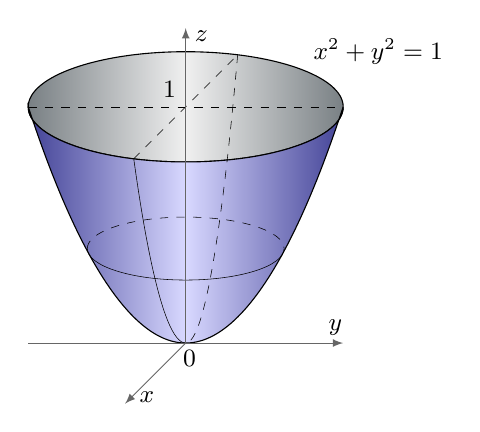
\begin{tikzpicture}
  \usetikzlibrary{arrows}
  \definecolor{insideo}{HTML}{798084}
  \definecolor{insidei}{HTML}{F0F0F0}
  \definecolor{outer}{HTML}{424296}
  \definecolor{inner}{HTML}{D8D8FF}
  \shadedraw [left color=insideo,right color=insideo,middle color=insidei] (0,3) ellipse (2 and 0.7);
  \shadedraw [left color=outer,right color=outer,middle color=inner]
  (2,3) arc (360:180:2 and 0.7) -- (-2,3) parabola bend (0,0) (2,3);
  \draw [dashed,line width=0.2pt] (-2,3) -- (2,3);
  \draw [dashed,line width=0.2pt] (-0.66,2.34) -- (0.66,3.66);
  \draw [line width=0.2pt] (-0.66,2.34) parabola [bend at end] (0,0);
  \draw [dashed,line width=0.2pt] (0.66,3.66) parabola [bend at end] (0,0);
  \draw [line width=0.2pt] (-1.25,1.2) arc (180:360:1.25 and 0.4);
  \draw [dashed,line width=0.2pt] (-1.25,1.2) arc (180:0:1.25 and 0.4);
  \draw [black!60,line width=0.3pt,-latex] (-2,0) -- (2,0,0);
  \draw [black!60,line width=0.3pt,-latex] (0,0) -- (0,4,0);
  \draw [black!60,line width=0.3pt,-latex] (0,0) -- (0,0,2);
  \pgfputat{\pgfpointxyz{1.9}{0.2}{0}}{\pgfbox[center,center]{\small $y$}};
  \pgfputat{\pgfpointxyz{0.2}{3.9}{0}}{\pgfbox[center,center]{\small $z$}};
  \pgfputat{\pgfpointxyz{0.2}{0}{1.8}}{\pgfbox[center,center]{\small $x$}};
  \pgfputat{\pgfpointxyz{0.05}{-0.2}{0}}{\pgfbox[center,center]{\small $0$}};
  \node [right] at (1.5,3.7) {\small $x^2 + y^2 = 1$};
  \node [above left] at (0,3) {\small $1$};
 \end{tikzpicture}
 }
 \par\noindent\emph{Solution:} Using vertical slices, we see that
 \begin{displaymath}
  V ~=~ \iint\limits_{R} (1 - z)\,dA ~=~ \iint\limits_{R} (1 - (x^2 + y^2 ))\,dA ~,
 \end{displaymath}
 where $R = \lbrace (x,y): x^2 + y^2 \le 1 \rbrace$ is the unit disk in $\Real{2}$
 (see Figure 3.5.2). In polar coordinates $(r,\theta)$
 we know that $x^2 + y^2 = r^2$ and that the unit disk $R$ is the set $R' = \lbrace (r,\theta):0 \le r \le 1, 0 \le
 \theta \le 2\pi \rbrace$. Thus,
 \begin{align*}
  V ~&=~ \int_0^{2\pi} \int_0^1 (1 - r^2 )\,r\,dr\,d\theta\\
   &=~ \int_0^{2\pi} \int_0^1 (r - r^3 )\,dr\,d\theta\\
   &=~ \int_0^{2\pi} \left( \tfrac{r^2}{2} - \tfrac{r^4}{4} \,\Big|_{r=0}^{r=1} \right) \,d\theta\\
   &=~ \int_0^{2\pi} \tfrac{1}{4} \,d\theta\\
   &=~ \frac{\pi}{2}
 \end{align*}
\end{exmp}
\hrule width \textwidth height 0.5pt

\begin{exmp}
 Find the volume $V$ inside the cone $z=\sqrt{x^2 + y^2}$ for $0 \le z \le 1$.\smallskip
 \piccaption[]{\quad $z=\sqrt{x^2 + y^2}$}\parpic[r]{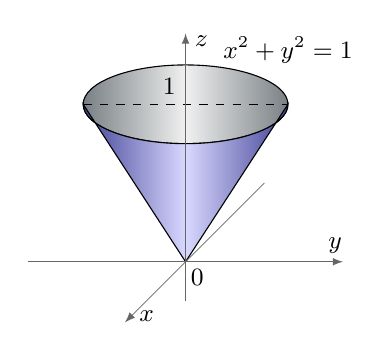
\begin{tikzpicture}
  \usetikzlibrary{arrows}
  \definecolor{insideo}{HTML}{798084}
  \definecolor{insidei}{HTML}{F0F0F0}
  \definecolor{outer}{HTML}{424296}
  \definecolor{inner}{HTML}{D8D8FF}
  \shadedraw [left color=insideo,right color=insideo,middle color=insidei] (1.3,2) arc (0:180:1.3 and .5) --
   (-1.3,2) arc (180:360:1.3 and .5);
  \shadedraw [left color=outer,right color=outer,middle color=inner] (0,0) -- (-1.3,2) arc (180:360:1.3 and .5)
   -- (0,0);
  \draw [dashed,line width=0.2pt] (-1.3,2) -- (1.3,2);
  \draw [black!60,line width=0.3pt,-latex] (-2,0) -- (2,0,0);
  \draw [black!60,line width=0.3pt,-latex] (1,1) -- (0,0,2);
  \draw [black!60,line width=0.3pt,-latex] (0,-0.5) -- (0,2.9,0);
  \pgfputat{\pgfpointxyz{1.9}{0.2}{0}}{\pgfbox[center,center]{\small $y$}};
  \pgfputat{\pgfpointxyz{0.2}{2.8}{0}}{\pgfbox[center,center]{\small $z$}};
  \pgfputat{\pgfpointxyz{0.2}{0}{1.8}}{\pgfbox[center,center]{\small $x$}};
  \pgfputat{\pgfpointxyz{0.15}{-0.2}{0}}{\pgfbox[center,center]{\small $0$}};
  \node [above] at (1.3,2.4) {\small $x^2 + y^2 = 1$};
  \node [above left] at (0,2) {\small $1$};
 \end{tikzpicture}
 }
 \par\noindent\emph{Solution:} Using vertical slices, we see that
 \begin{displaymath}
  V ~=~ \iint\limits_{R} (1 - z)\,dA ~=~ \iint\limits_{R} \left( 1 - \sqrt{x^2 + y^2} \right) \,dA ~,
 \end{displaymath}
 where $R = \lbrace (x,y): x^2 + y^2 \le 1 \rbrace$ is the unit disk in $\Real{2}$\\
 (see Figure 3.5.3). In polar coordinates $(r,\theta)$
 we know\\that $\sqrt{x^2 + y^2} = r$ and that the unit disk $R$ is the set\\$R' = \lbrace (r,\theta):0 \le r \le 1, 0
 \le \theta \le 2\pi \rbrace$. Thus,
 \begin{align*}
  V ~&=~ \int_0^{2\pi} \int_0^1 (1 - r)\,r\,dr\,d\theta\\
   &=~ \int_0^{2\pi} \int_0^1 (r - r^2 )\,dr\,d\theta\\
   &=~ \int_0^{2\pi} \left( \tfrac{r^2}{2} - \tfrac{r^3}{3} \,\Big|_{r=0}^{r=1} \right) \,d\theta\\
   &=~ \int_0^{2\pi} \tfrac{1}{6} \,d\theta\\
   &=~ \frac{\pi}{3}
 \end{align*}
\end{exmp}
\hrule width \textwidth height 0.5pt
\medskip

In a similar fashion, it can be shown (see Exercises 5--6) that triple integrals in cylindrical and spherical coordinates
take the following forms:

\smallskip
\statecomment{
 \textbf{Triple Integral in Cylindrical Coordinates}\index{triple integral!cylindrical coordinates}
 \begin{equation}\label{eqn:cylinderint}
  \iiint\limits_{S} f(x,y,z)\,dx\,dy\,dz ~=~ \iiint\limits_{S'} f(r\cos \theta,r\sin \theta,z)\,r\,dr\,d\theta\,dz ~,
 \end{equation}
 where the mapping $x=r\cos \theta$, $y=r\sin \theta$, $z=z$ maps the solid $S'$ in 
 $r\theta z$-space onto the solid $S$ in $xyz$-space in a one-to-one manner.
}

\smallskip
\statecomment{
 \textbf{Triple Integral in Spherical Coordinates}\index{triple integral!spherical coordinates}
 \begin{equation}\label{eqn:sphereint}
  \iiint\limits_{S} f(x,y,z)\,dx\,dy\,dz ~=~
  \iiint\limits_{S'} f(\rho\sin \phi\,\cos \theta,\rho\sin \phi\,\sin \theta,\rho\cos \phi)
  \,\rho^2 \,\sin \phi \,d\rho\,d\phi\,d\theta ~,
 \end{equation}
 where the mapping $x=\rho\sin \phi\,\cos \theta$, $y=\rho\sin \phi\,\sin \theta$, $z=\rho\cos \phi$ maps the solid
 $S'$ in  $\rho\phi\theta$-space onto the solid $S$ in $xyz$-space in a one-to-one manner.
}

\begin{exmp}\label{exmp:volsphere}
 For $a > 0$, find the volume $V$ inside the sphere $S = x^2 + y^2 + z^2 = a^2$.\smallskip
 \par\noindent\emph{Solution:} We see that $S$ is the set $\rho = a$ in spherical coordinates, so
 \begin{align*}
  V ~&=~ \iiint\limits_{S} 1\,dV
   ~=~ \int_0^{2\pi} \int_0^{\pi} \int_0^a 1 \,\rho^2 \,\sin \phi \,d\rho\,d\phi\,d\theta\\
   &=~ \int_0^{2\pi} \int_0^{\pi} \left( \frac{\rho^3}{3}\,\Big|_{\rho=0}^{\rho=a}\right)\,\sin \phi \,d\phi\,d\theta
   ~=~ \int_0^{2\pi} \int_0^{\pi} \frac{a^3}{3}\,\sin \phi\,d\phi\,d\theta\\
   &=~ \int_0^{2\pi} \left(  -\frac{a^3}{3}\,\cos \phi\,\Big|_{\phi=0}^{\phi=\pi} \right) \,d\theta
   ~=~ \int_0^{2\pi} \frac{2a^3}{3}\,d\theta
   ~=~ \frac{4\pi a^3}{3} ~.
 \end{align*}
\end{exmp}
\startexercises\label{sec3dot5}
\probs{A}
\begin{enumerate}[\bfseries 1.]
 \item Find the volume $V$ inside the paraboloid $z=x^2 + y^2$ for $0 \le z \le 4$.
 \item Find the volume $V$ inside the cone $z=\sqrt{x^2 + y^2}$ for $0 \le z \le 3$.
\suspend{enumerate}
\probs{B}
\resume{enumerate}[{[\bfseries 1.]}]
 \item Find the volume $V$ of the solid inside both $x^2 + y^2 + z^2 = 4$ and $x^2 + y^2 = 1$.
 \item Find the volume $V$ inside both the sphere $x^2 + y^2 + z^2 = 1$ and the cone $z=\sqrt{x^2 + y^2}$.
 \begin{multicols}{2}
  \item Prove formula (\ref{eqn:cylinderint}).
  \item Prove formula (\ref{eqn:sphereint}).
 \end{multicols}
 \item Evaluate $\iint\limits_{R} \sin \left( \frac{x+y}{2} \right)\,\cos \left( \frac{x-y}{2} \right)\,dA$, where $R$
  is the triangle with vertices $(0,0)$, $(2,0)$ and $(1,1)$. (\emph{Hint: Use the change of variables
  $u=(x+y)/2$, $v=(x-y)/2$.})
 \item Find the volume of the solid bounded by $z=x^2 + y^2$ and $z^2 = 4(x^2 + y^2)$.
 \item Find the volume inside the elliptic cylinder $\frac{x^2}{a^2} + \frac{y^2}{b^2} \le 1$ for $0\le z\le 2$.
\suspend{enumerate}
\probs{C}
\resume{enumerate}[{[\bfseries 1.]}]
 \item Show that the volume inside the ellipsoid $\frac{x^2}{a^2} + \frac{y^2}{b^2} + \frac{z^2}{c^2} = 1$ is
  $\tfrac{4\pi abc}{3}$. (\emph{Hint: Use the change of variables $x=au$, $y=bv$, $z=cw$, then consider Example
  \ref{exmp:volsphere}.})\index{ellipsoid}
\item Show that 
\[\int\limits_{-\infty}^{+\infty}\,\int\limits_{-\infty}^{+\infty}f(x,y)\,dx\,dy
=
\int\limits_{-\infty}^{+\infty}\,\int\limits_{-\infty}^{+\infty}f(x+y,x+2y)\,dx\,dy\]
For any smooth function $f(x,y)$ which vanishes outside of a bounded region in the plane.
\end{enumerate}
\newpage
%Begin Section 3.6
\section{Application: Center of Mass}
\piccaption[]{\quad Center of mass of $R$}\parpic[r]{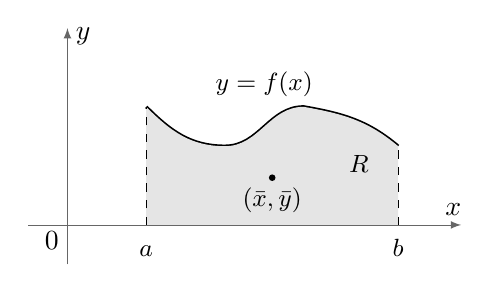
\begin{tikzpicture}[every node/.style={font=\small}]
  \usetikzlibrary{arrows}
  \draw [black,line width=1.2pt] (4.2,1) to[out=140,in=-10] (3,1.5) to[out=180,in=0] (2,1) to[out=180,in=-45] (1,1.5);
  \fill [fill=black!10] (4.2,1) to[out=140,in=-10] (3,1.5) to[out=180,in=0] (2,1) to[out=180,in=-45] (1,1.5) --
   (1,0) -- (4.2,0) -- (4.2,1);
  \draw [black!60,line width=0.3pt,-latex,anchor=base] (-0.5,0) -- (5,0)
    node[black,shift={(0,-0.4)}] at (1,0) {$a$}
    node[black,shift={(0,-0.4)}] at (4.2,0) {$b$};
  \draw [black!60,line width=0.3pt,-latex] (0,-0.5) -- (0,2.5);
  \pgfputat{\pgfpointxyz{4.9}{0.2}{0}}{\pgfbox[center,center]{$x$}}
  \pgfputat{\pgfpointxyz{0.2}{2.4}{0}}{\pgfbox[center,center]{$y$}}
  \pgfputat{\pgfpointxyz{-0.2}{-0.2}{0}}{\pgfbox[center,center]{$0$}}
  \node [above] at (2.5,1.5) {$y = f(x)$};
  \node [below] at (3.7,1) {$R$};
  \fill (2.6,0.6) circle (1.2pt);
  \node [below] at (2.6,0.6) {$(\bar{x},\bar{y})$};
  \draw [dashed] (1,0) -- (1,1.5);
  \draw [dashed] (4.2,0) -- (4.2,1);
 \end{tikzpicture}
}
\par\noindent Recall from single-variable calculus that for a region\index{center of mass}
$R = \lbrace (x,y): a \le x \le b, 0 \le y \le f(x) \rbrace$ in $\Real{2}$ that represents a thin,
flat plate (see Figure 3.6.1), where $f(x)$ is a\index{$\bar{x}$}\index{$\bar{y}$}\index{$M_x$, $M_y$}
continuous function on $\ival{a}{b}$, the \emph{center of mass} of $R$ has coordinates $(\bar{x},\bar{y})$ given by
\begin{displaymath}
 \bar{x} = \frac{M_y}{M} \quad \text{and} \quad \bar{y} = \frac{M_x}{M} ~,
\end{displaymath}
where\picskip{0}
\begin{equation}\label{eqn:moment1}
 M_x = \int_a^b \frac{(f(x))^2}{2}\,dx ~, \quad M_y = \int_a^b x f(x)\,dx ~, \quad M = \int_a^b f(x)\,dx ~,
\end{equation}
assuming that $R$ has \emph{uniform density}, i.e the \emph{mass} of $R$ is uniformly distributed over the region. In
this case the area $M$ of the region is considered the mass of $R$ (the density is constant, and taken as $1$ for
simplicity).\index{density}\index{$\delta(x,y)$}\index{lamina}\index{uniform density}\index{moment}\index{mass}

In the general case where the density of a region (or \emph{lamina}) $R$ is a continuous function $\delta = \delta(x,y)$
of the coordinates
$(x,y)$ of points inside $R$ (where $R$ can be \emph{any} region in $\Real{2}$) the coordinates $(\bar{x},\bar{y})$ of
the center of mass of $R$ are given by
\begin{equation}\label{eqn:center2}
 \bar{x} = \frac{M_y}{M} \quad \text{and} \quad \bar{y} = \frac{M_x}{M} ~,
\end{equation}
where
\begin{equation}\label{eqn:moment2}
 M_y = \iint\limits_{R} x\delta(x,y)\,dA ~, \quad M_x = \iint\limits_{R} y\delta(x,y)\,dA ~,
 \quad M = \iint\limits_{R} \delta(x,y)\,dA ~,
\end{equation}
The quantities $M_x$ and $M_y$ are called the \emph{moments} (or \emph{first moments}) of the region $R$ about
the $x$-axis and $y$-axis, respectively.
The quantity $M$ is the mass of the region $R$. To see this, think of taking a small rectangle inside $R$ with
dimensions $\Delta x$ and $\Delta y$ close to $0$. The mass of that rectangle is approximately
$\delta(x_* ,y_* ) \Delta x \, \Delta y$, for some point $(x_* ,y_* )$ in that rectangle. Then the mass of $R$ is the
limit of the sums of the masses of all such rectangles inside $R$ as the diagonals of the rectangles approach $0$, which
is the double integral $\iint\limits_{R} \delta(x,y)\,dA$.

Note that the formulas in (\ref{eqn:moment1}) represent a special case when
$\delta(x,y) = 1$ throughout $R$ in the formulas in (\ref{eqn:moment2}).

\medskip
\hrule width \textwidth height 0.5pt
\begin{exmp}
 Find the center of mass of the region $R = \lbrace (x,y): 0 \le x \le 1,~ 0 \le y \le 2x^2 \rbrace$,
 if the density function at $(x,y)$ is $\delta(x,y) = x+y$.\smallskip
 \piccaption[]{}\parpic[r]{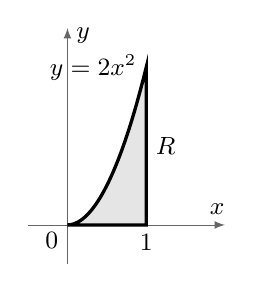
\begin{tikzpicture}
   \usetikzlibrary{arrows}
   \draw [black!60,line width=0.3pt,-latex] (-0.5,0) -- (2,0);
   \draw [black!60,line width=0.3pt,-latex] (0,-0.5) -- (0,2.5);
   \pgfputat{\pgfpointxyz{1.9}{0.2}{0}}{\pgfbox[center,center]{\small $x$}}
   \pgfputat{\pgfpointxyz{0.2}{2.4}{0}}{\pgfbox[center,center]{\small $y$}}
   \pgfputat{\pgfpointxyz{-0.2}{-0.2}{0}}{\pgfbox[center,center]{\small $0$}}
   \filldraw [black,line width=1.2pt,fill=black!10] (0,0) parabola (1,2) -- (1,0) -- (0,0);
   \node [left] at (1,2) {\small $y = 2x^2$};
   \node [right] at (1,1) {\small $R$};
   \node [below] at (1,0) {\small $1$};
  \end{tikzpicture}}
 \par\noindent \emph{Solution:} The region $R$ is shown in Figure 3.6.2. We have
 \begin{align*}
  M ~&=~ \iint\limits_{R} \delta(x,y)\,dA\\
   &=~ \int_0^1 \int_0^{2x^2} (x+y)\,dy\,dx\\
   &=~ \int_0^1 \left( xy + \frac{y^2}{2} \,\Bigg|_{y=0}^{y=2x^2} \right) \,dx\\
   &=~ \int_0^1 ( 2x^3 + 2x^4 ) \,dx\\
   &=~ \frac{x^4}{2} + \frac{2x^5}{5} \,\Bigg|_0^1 ~=~ \frac{9}{10}
 \end{align*}
 and\picskip{0}
 \begin{alignat*}{2}
  M_x ~&=~ \iint\limits_{R} y\delta(x,y)\,dA & M_y ~&=~ \iint\limits_{R} x\delta(x,y)\,dA\\
  &=~ \int_0^1 \int_0^{2x^2} y(x+y)\,dy\,dx \qquad\qquad\qquad & \phantom{M_y} &=~ \int_0^1 \int_0^{2x^2} x(x+y)\,dy\,dx\\
  &=~ \int_0^1 \left( \frac{xy^2}{2} + \frac{y^3}{3} \,\Bigg|_{y=0}^{y=2x^2} \right) \,dx & \phantom{M_y}
  &=~ \int_0^1 \left( x^2 y + \frac{xy^2}{2} \,\Bigg|_{y=0}^{y=2x^2} \right) \,dx\\
  &=~ \int_0^1 ( 2x^5 + \frac{8x^6}{3} ) \,dx & \phantom{M_y} &=~ \int_0^1 ( 2x^4 + 2x^5 ) \,dx\\
  &=~ \frac{x^6}{3} + \frac{8x^7}{21} \,\Bigg|_0^1 ~=~ \frac{5}{7} & \phantom{M_y}
  &=~ \frac{2x^5}{5} + \frac{x^6}{3} \,\Bigg|_0^1 ~=~ \frac{11}{15} ~,
 \end{alignat*}
 so the center of mass $(\bar{x},\bar{y})$ is given by
 \begin{displaymath}
  \bar{x} ~=~ \frac{M_y}{M} ~=~ \frac{11/15}{9/10} ~=~ \frac{22}{27} ~, \quad
  \bar{y} ~=~ \frac{M_x}{M} ~=~ \frac{5/7}{9/10} ~=~ \frac{50}{63} ~.
 \end{displaymath}
 Note how this center of mass is a little further towards the upper corner of the region $R$ than when the density is
 uniform (use the formulas in (\ref{eqn:moment1}) to show that $(\bar{x},\bar{y}) =
 \left( \frac{3}{4},\frac{3}{5} \right)$ in that case). This makes sense since the density
 function $\delta(x,y) = x+y$ increases as $(x,y)$ approaches that upper corner, where there is quite a bit of area.
\end{exmp}
\hrule width \textwidth height 0.5pt
\medskip

In the special case where the density function $\delta(x,y)$ is a constant function on the region $R$, the center of
mass $(\bar{x},\bar{y})$ is called the \emph{centroid} of $R$.\index{centroid}

The formulas for the center of mass of a region in $\Real{2}$ can be generalized to a solid $S$ in $\Real{3}$.
Let $S$ be a solid with a continuous mass density function $\delta(x,y,z)$ at any point $(x,y,z)$ in $S$. Then the
center of mass of $S$ has coordinates $(\bar{x},\bar{y},\bar{z})$, where\index{$\bar{z}$}\index{moment}\index{$M_{xy}$,
$M_{xz}$, $M_{yz}$}
\begin{equation}\label{eqn:center3}
 \bar{x} ~=~ \frac{M_{yz}}{M} ~,\quad \bar{y} ~=~ \frac{M_{xz}}{M} ~,\quad \bar{z} ~=~ \frac{M_{xy}}{M} ~,
\end{equation}
where
\begin{gather}\label{eqn:moment3}
 M_{yz} ~=~ \iiint\limits_{S} x\delta(x,y,z)\,dV ~, \quad M_{xz} ~=~ \iiint\limits_{S} y\delta(x,y,z)\,dV ~, \quad
 M_{xy} ~=~ \iiint\limits_{S} z\delta(x,y,z)\,dV ~,\\M ~=~ \iiint\limits_{S} \delta(x,y,z)\,dV ~.
\end{gather}
In this case, $M_{yz}$, $M_{xz}$ and $M_{xy}$ are called the \emph{moments} (or \emph{first moments}) of $S$
around the $yz$-plane, $xz$-plane and $xy$-plane, respectively. Also, $M$ is the mass of $S$.

\medskip
\hrule width \textwidth height 0.5pt
\begin{exmp}\label{exmp:uspherecenter}
 Find the center of mass of the solid $S = \lbrace (x,y,z): z \ge 0,~ x^2 + y^2 + z^2 \le a^2 \rbrace$,
 if the density function at $(x,y,z)$ is $\delta(x,y,z) = 1$.\smallskip
 \piccaption[]{}\parpic[r]{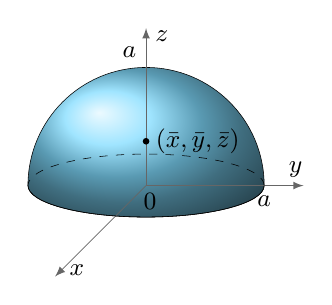
\begin{tikzpicture}
  \usetikzlibrary{arrows}
  \definecolor{spherecolor}{HTML}{80DCFF}
  \definecolor{planecolor}{HTML}{FFB270}
  \shadedraw [line width=0.2pt,ball color=spherecolor] (-1.5,0) arc (180:360:1.5 and 0.4) arc (0:180:1.5);
  \draw [black!60,line width=0.3pt,-latex] (0,0) -- (2,0,0);
  \draw [black!60,line width=0.3pt,-latex] (0,0) -- (0,2,0);
  \draw [black!60,line width=0.3pt,-latex] (0,0) -- (0,0,3);
  \pgfputat{\pgfpointxyz{1.9}{0.2}{0}}{\pgfbox[center,center]{\small $y$}};
  \pgfputat{\pgfpointxyz{0.2}{1.9}{0}}{\pgfbox[center,center]{\small $z$}};
  \pgfputat{\pgfpointxyz{0.2}{0}{2.8}}{\pgfbox[center,center]{\small $x$}};
  \pgfputat{\pgfpointxyz{0.05}{-0.2}{0}}{\pgfbox[center,center]{\small $0$}};
  \draw [line width=0.2pt] (-1.5,0) arc (180:360:1.5 and 0.4);
  \draw [dashed,line width=0.2pt] (1.5,0) arc (0:180:1.5 and 0.4);
  \node [below] at (1.5,0) {\small $a$};
  \node [right] at (0,0.5625) {\small $(\bar{x},\bar{y},\bar{z})$};
  \node [above left] at (0,1.5) {\small $a$};
  \fill (0,0.5625) circle (1.2pt);
 \end{tikzpicture}
 }
 \par\noindent \emph{Solution:} 
 The solid $S$ is just the upper hemisphere inside the sphere of radius $a$ centered at
 the origin (see Figure 3.6.3). 
 So since the density function is a constant and $S$ is symmetric about the $z$-axis,
 then it is clear that $\bar{x}=0$ and $\bar{y}=0$, so we need only find $\bar{z}$. 
 We have
 \begin{displaymath}
  M ~=~ \iiint\limits_{S} \delta(x,y,z)\,dV = \iiint\limits_{S} 1\,dV = Volume(S).
 \end{displaymath}
 But since the volume of $S$ is half the volume of the sphere of radius $a$, which we know by Example
 \ref{exmp:volsphere} is $\frac{4\pi a^3}{3}$, then $M = \frac{2\pi a^3}{3}$. And
 \begin{align*}
  M_{xy} ~&=~ \iiint\limits_{S} z\delta(x,y,z)\,dV\\
  &=~ \iiint\limits_{S} z\,dV ~~,~\text{which in spherical coordinates is}\\
  &=~ \int_0^{2\pi} \int_0^{\pi /2} \int_0^a (\rho\,\cos \phi )\,\rho^2 \,\sin \phi \,d\rho\,d\phi\,d\theta\\[8pt]
  &=~ \int_0^{2\pi} \int_0^{\pi /2} \,\sin \phi \,\cos \phi \left( \int_0^a \rho^3 \,d\rho \right) \,d\phi\,d\theta\\[8pt]
  &=~ \int_0^{2\pi} \int_0^{\pi /2} \tfrac{a^4}{4}\,\sin \phi\,\cos \phi\,d\phi\,d\theta\\[8pt]
  M_{xy} ~&=~ \int_0^{2\pi} \int_0^{\pi /2} \tfrac{a^4}{8}\,\sin 2\phi\,d\phi\,d\theta ~~~\text{(since $\sin 2\phi =
  2\sin \phi \, \cos \phi$)}\\[8pt]
  &=~ \int_0^{2\pi} \left(  -\tfrac{a^4}{16}\,\cos 2\phi\,\Big|_{\phi=0}^{\phi=\pi /2} \right) \,d\theta\\[8pt]
  &=~ \int_0^{2\pi} \tfrac{a^4}{8}\,d\theta\\
  &=~ \frac{\pi a^4}{4}~,
 \end{align*}
 so
 \begin{displaymath}
  \bar{z} ~=~ \frac{M_{xy}}{M} ~=~ \frac{\tfrac{\pi a^4}{4}}{\tfrac{2\pi a^3}{3}} ~=~ \frac{3a}{8} ~.
 \end{displaymath}
 Thus, the center of mass of $S$ is $(\bar{x},\bar{y},\bar{z}) = \left( 0,0,\frac{3a}{8} \right)$.
\end{exmp}
\startexercises\label{sec3dot6}
\probs{A}
\par\noindent For Exercises 1--5, find the center of mass of the region $R$ with the given density function
$\delta(x,y)$.
\begin{enumerate}[\bfseries 1.]
 \item $R = \lbrace (x,y): 0 \le x \le 2,~ 0 \le y \le 4~ \rbrace$, $\delta(x,y) = 2y$
 \item $R = \lbrace (x,y): 0 \le x \le 1,~ 0 \le y \le x^2 \rbrace$, $\delta(x,y) = x+y$
 \item $R = \lbrace (x,y): y \ge 0, ~x^2 + y^2 \le a^2 \rbrace$, $\delta(x,y) = 1$
 \item $R = \lbrace (x,y): y \ge 0,~ x \ge 0, ~ 1 \le x^2 + y^2 \le 4~ \rbrace$, $\delta(x,y) = \sqrt{x^2 + y^2}$
 \item $R = \lbrace (x,y): y \ge 0, ~x^2 + y^2 \le 1~ \rbrace$, $\delta(x,y) = y$
\suspend{enumerate}
\probs{B}
\par\noindent For Exercises 6--10, find the center of mass of the solid $S$ with the given density function
$\delta(x,y,z)$.
\resume{enumerate}[{[\bfseries 1.]}]
 \item $S = \lbrace (x,y,z): 0 \le x \le 1,~ 0 \le y \le 1,~ 0 \le z \le 1~ \rbrace$, $\delta(x,y,z) = xyz$
 \item $S = \lbrace (x,y,z): z \ge 0,~ x^2 + y^2 + z^2 \le a^2 \rbrace$, $\delta(x,y,z) = x^2 + y^2 + z^2$
 \item $S = \lbrace (x,y,z): x \ge 0,~ y \ge 0,~ z \ge 0, ~x^2 + y^2 + z^2 \le a^2 \rbrace$, $\delta(x,y,z) = 1$
 \item $S = \lbrace (x,y,z): 0 \le x \le 1,~ 0 \le y \le 1,~ 0 \le z \le 1~ \rbrace$, $\delta(x,y,z) = x^2 + y^2 + z^2$
 \item $S = \lbrace (x,y,z): 0 \le x \le 1,~ 0 \le y \le 1,~ 0 \le z \le 1 - x - y \rbrace$, $\delta(x,y,z) = 1$
\suspend{enumerate}
\probs{C}
\resume{enumerate}[{[\bfseries 1.]}]
\item Let $F$ be a figure in the upper half-plane;
denote as $(x_0,y_0)$ its center of mass 
and as $A$ its the area.
Show that 
\[2\pi A y_0\]
is the volume of the body of revolution obtained by rotating $F$ around $x$-axis.
\end{enumerate}
\newpage
%Begin Section 3.7
\section{Application: Probability and Expected Value}
In this section we will briefly discuss some applications of multiple integrals in the field of
probability theory. In particular we will see ways in which multiple integrals can be used to calculate
\emph{probabilities} and \emph{expected values}.\medskip

\par\noindent\textbf{\large{Probability}}\normalsize\smallskip

Suppose that you have a standard six-sided (fair) die, and you let a variable $X$ represent the value rolled. Then the
\emph{probability} of rolling a $3$, written as $P(X=3)$, is $\frac{1}{6}$, since there are six sides on the die and
each one is equally likely to be rolled, and hence in particular the $3$ has a one out of six chance of being rolled.
Likewise the probability of rolling \emph{at most} a $3$, written as $P(X \le 3)$, is $\frac{3}{6} = \frac{1}{2}$,
since of the six numbers on the die, there are three equally likely numbers ($1$, $2$, and $3$) that are less than or
equal to $3$. Note that $P(X \le 3) = P(X=1) + P(X=2) + P(X=3)$. We call $X$ a \emph{discrete random variable} on the
\emph{sample space} (or \emph{probability space}) $\Omega$ consisting of all possible outcomes. In our case,
$\Omega = \lbrace 1,2,3,4,5,6 \rbrace$.
An \emph{event} $A$ is a subset of the sample space. For example, in the case of the die, the event $X \le 3$ is the set
$\lbrace 1,2,3 \rbrace$.\index{probability}\index{random variable}\index{sample space}

Now let $X$ be a variable representing a random real number in the interval $(0,1)$. 
Note that for any real number
$x$ in $(0,1)$, it makes no sense to consider $P(X=x)$ since it \emph{must} be $0$ (why?). 
Instead, we consider the probability $P(X \le x)$, which is given by $P(X \le x) = x$. The reasoning is this: the interval $(0,1)$ has length $1$,
and for $x$ in $(0,1)$ the interval $(0,x)$ has length $x$. So since $X$ represents a \emph{random} number in $(0,1)$,
and hence is \emph{uniformly distributed} over $(0,1)$, then\index{uniformly distributed}
\begin{displaymath}
 P(X \le x) ~=~ \frac{\text{length of $(0,x)$}}{\text{length of $(0,1)$}} ~=~ \frac{x}{1} ~=~ x ~.
\end{displaymath}
We call $X$ a \emph{continuous random variable} on the \emph{sample space} $\Omega = (0,1)$. An \emph{event} $A$ is a
subset of the sample space. For example, in our case the event $X \le x$ is the set $(0,x)$.

In the case of a discrete random variable, we saw how the probability of an event was the \emph{sum} of the
probabilities of the individual outcomes comprising that event 
(for instance, $P(X \le 3) = P(X=1) + P(X=2) + P(X=3)$ in the die example). 
For a continuous random variable, the probability of an event will instead be the \emph{integral} of a
function, which we will now describe.

Let $X$ be a continuous real-valued random variable on a sample space $\Omega$ in $\mathbb{R}$. For simplicity, let
$\Omega= (a,b)$. Define the \emph{distribution function} $F$ of $X$ as\index{distribution function}
\begin{align}\label{eqn:distribfcn}
 F(x) ~&=~ P(X \le x)~, \quad \text{for $-\infty < x < \infty$}\\
  &=~ \begin{cases}
   1, &\text{for $x \ge b$}\\
   P(X \le x), &\text{for $a < x < b$}\\
   0, &\text{for $x \le a~$.}
  \end{cases}
\end{align}
Suppose that there is a nonnegative, continuous real-valued function $f$ on $\mathbb{R}$ such that
\begin{equation}\label{eqn:pdf}
 F(x) ~=~ \int_{-\infty}^x f(y)\,dy~, \quad \text{for $-\infty < x < \infty$} ~,
\end{equation}
and
\begin{equation}\label{eqn:pdfint}
\int_{-\infty}^{\infty} f(x)\,dx ~=~ 1 ~.
\end{equation}
Then we call $f$ the \emph{probability density function}  for $X$. 
We thus have
\begin{equation}\label{eqn:pdfprob}
 P(X \le x) ~=~ \int_{a}^x f(y)\,dy~, \quad \text{for $a < x < b$} ~.
\end{equation}
Also, by the Fundamental Theorem of Calculus, we have\index{probability density function}
\begin{equation}\label{eqn:pdfderiv}
 F\,'(x) ~=~ f(x)~, \quad \text{for $-\infty < x < \infty$.}
\end{equation}
\hrule width \textwidth height 0.5pt
\begin{exmp}\label{exmp:unifdistrib}
 Let $X$ represent a randomly selected real number in the interval $(0,1)$. We say that $X$ 
 has the \emph{uniform distribution}\index{uniform distribution} on $(0,1)$, with distribution function
  \begin{equation}
   F(x) ~=~ P(X \le x)
   ~=~ \begin{cases}
   1, &\text{for $x \ge 1$}\\
   x, &\text{for $0 < x < 1$}\\
   0, &\text{for $x \le 0~$,}
  \end{cases}
 \end{equation}
 and probability density function
 \begin{equation}
   f(x) ~=~ F\,'(x)
   ~=~ \begin{cases}
   1, &\text{for $0 < x < 1$}\\
   0, &\text{elsewhere.}
  \end{cases}
 \end{equation}
 In general, if $X$ represents a randomly selected real number in an interval $(a,b)$, then $X$ has the uniform
 distribution function
 \begin{equation}
   F(x) ~=~ P(X \le x)
   ~=~ \begin{cases}
   1, &\text{for $x \ge b$}\\
   \frac{x}{b-a}, &\text{for $a < x < b$}\\
   0, &\text{for $x \le a~$,}
  \end{cases}
 \end{equation}
 and probability density function
 \begin{equation}
   f(x) ~=~ F\,'(x)
   ~=~ \begin{cases}
   \frac{1}{b-a}, &\text{for $a < x < b$}\\
   0, &\text{elsewhere.}
  \end{cases}
 \end{equation}
\end{exmp}
\hrule width \textwidth height 0.5pt

\begin{exmp}\label{exmp:normaldistrib}
 A famous distribution function is given by the \emph{standard normal distribution}, whose probability density function
 $f$ is\index{standard normal distribution}\index{distribution function!normal}
 \begin{equation}\label{eqn:normalpdf}
  f(x) ~=~ \frac{1}{\sqrt{2\pi}} e^{-x^2 /2}~, \quad \text{for $-\infty < x < \infty$.}
 \end{equation}
 This is often called a ``bell curve'', and is used widely in statistics. 
 Since we are claiming that $f$ is a probability density function,
 we \emph{should} have
 \begin{equation}
  \int_{-\infty}^{\infty} \frac{1}{\sqrt{2\pi}} e^{-x^2 /2}\,dx ~=~ 1
 \end{equation}
 by formula (\ref{eqn:pdfint}), which is equivalent to
 \begin{equation}
  \int_{-\infty}^{\infty} e^{-x^2 /2}\,dx ~=~ \sqrt{2\pi} ~.
 \end{equation}
 We can use a double integral in polar coordinates to verify this integral. First,
 \begin{align*}
  \int_{-\infty}^{\infty} \int_{-\infty}^{\infty} e^{-(x^2 + y^2 )/2}\,dx\,dy ~&=~
  \int_{-\infty}^{\infty} e^{-y^2 /2} \left( \int_{-\infty}^{\infty} e^{-x^2 /2}\,dx \right) \,dy\\[6pt]
  &=~ \left( \int_{-\infty}^{\infty} e^{-x^2 /2}\,dx \right)\,\left( \int_{-\infty}^{\infty} e^{-y^2 /2}\,dy \right)\\[6pt]
  &=~ \left( \int_{-\infty}^{\infty} e^{-x^2 /2}\,dx \right)^2
 \end{align*}
 since the same function is being integrated twice in the middle equation, just with different variables. But using
 polar coordinates, we see that
 \begin{align*}
  \int_{-\infty}^{\infty} \int_{-\infty}^{\infty} e^{-(x^2 + y^2 )/2}\,dx\,dy
  ~&=~ \int_0^{2\pi} \int_0^{\infty} e^{-r^2 /2}\,r\,dr\,d\theta\\[6pt]
  &=~ \int_0^{2\pi} \left( -e^{-r^2 /2} \,\Bigg|_{r=0}^{r=\infty} \,\right)\,d\theta\\[6pt]
  &=~ \int_0^{2\pi} (0 - (-e^0))\,d\theta = \int_0^{2\pi} 1\,d\theta ~=~ 2\pi ~,
 \end{align*}
 and so
 \begin{align*}
  \left( \int_{-\infty}^{\infty} e^{-x^2 /2}\,dx \right)^2 ~&=~ 2\pi ~~,~\text{and hence}\\[6pt]
  \int_{-\infty}^{\infty} e^{-x^2 /2}\,dx ~&=~ \sqrt{2\pi} ~.
 \end{align*}
\end{exmp}
\hrule width \textwidth height 0.5pt
\smallskip
In addition to individual random variables, we can consider \emph{jointly distributed} random variables. For this, we
will let $X$, $Y$ and $Z$ be three real-valued continuous random variables defined on the same sample space
$\Omega$ in $\mathbb{R}$ (the discussion for two random variables is similar). Then the \emph{joint distribution
function} $F$ of $X$, $Y$ and $Z$ is given by\index{joint distribution}\index{distribution function!joint}
\begin{equation}
 F(x,y,z) ~=~ P(X \le x,~Y \le y,~Z \le z)~, \quad \text{for $-\infty < x,y,z < \infty$.}
\end{equation}
If there is a nonnegative, continuous real-valued function $f$ on $\Real{3}$ such that
\begin{equation}\label{eqn:pdf3}
 F(x,y,z) 
 ~=~ 
 \int_{-\infty}^z \,\,
 \int_{-\infty}^y \,\,\int_{-\infty}^x 
 f(u,v,w)\,du\,dv\,dw~,
 \quad \text{for $-\infty < x,y,z < \infty$}
\end{equation}
and
\begin{equation}\label{eqn:pdfint3}
\int_{-\infty}^{\infty}\,\, \int_{-\infty}^{\infty}\,\, \int_{-\infty}^{\infty} f(x,y,z)\,dx\,dy\,dz ~=~ 1 ~,
\end{equation}
then we call $f$ the \emph{joint probability density function}  for $X$, $Y$ and $Z$.
In general, for $\ssub{a}{1} < \ssub{b}{1}$, $\ssub{a}{2} < \ssub{b}{2}$, $\ssub{a}{3} < \ssub{b}{3}$, we have
\begin{equation}\label{eqn:pdfprob3}
 P(\ssub{a}{1} < X \le \ssub{b}{1},~\ssub{a}{2} < Y \le \ssub{b}{2},~\ssub{a}{3} < Z \le \ssub{b}{3}) ~=~
 \int_{\ssub{a}{3}}^{\ssub{b}{3}}\int_{\ssub{a}{2}}^{\ssub{b}{2}}\int_{\ssub{a}{1}}^{\ssub{b}{1}} f(x,y,z)\,dx\,dy\,dz~,
\end{equation}
with the $\le$ and $<$ symbols interchangeable in any combination. 
A triple integral, then, can be thought of as
representing a probability (for a function $f$ which is a probability density function).

\medskip
\hrule width \textwidth height 0.5pt
\begin{exmp}\label{exmp:quadprob}
 Let $a$, $b$, and $c$ be real numbers selected randomly from the interval $(0,1)$. What is the probability that the
 equation $ax^2 + bx + c = 0$ has at least one real solution $x$?\smallskip

 \piccaption[]{\quad Region $R = \ssub{R}{1} \cup \ssub{R}{2}$}\parpic[r]{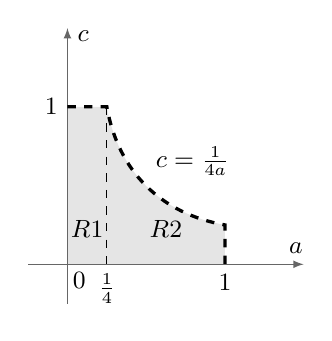
\begin{tikzpicture}
  \usetikzlibrary{arrows}
  \fill [fill=black!10] (0,2) -- (0.5,2) to[out=-80,in=170] (2,0.5) -- (2,0) -- (0,0) -- (0,2);
  \draw [black!60,line width=0.3pt,-latex] (-0.5,0) -- (3,0,0);
  \draw [black!60,line width=0.3pt,-latex] (0,-0.5) -- (0,3,0);
  \pgfputat{\pgfpointxyz{2.9}{0.2}{0}}{\pgfbox[center,center]{\small $a$}};
  \pgfputat{\pgfpointxyz{0.2}{2.9}{0}}{\pgfbox[center,center]{\small $c$}};
  \pgfputat{\pgfpointxyz{0.15}{-0.2}{0}}{\pgfbox[center,center]{\small $0$}};
  \node [above right] at (1,1) {\small $c=\frac{1}{4a}$};
  \node [left] at (0,2) {\small $1$};
  \node [below] at (2,0) {\small $1$};
  \node [below] at (0.5,0) {\small $\frac{1}{4}$};
  \node at (0.25,0.45) {\small $\ssub{R}{1}$};
  \node at (1.25,0.45) {\small $\ssub{R}{2}$};
  \draw [black,line width=1.2pt,dashed] (0,2) -- (0.5,2) to[out=-80,in=170] (2,0.5) -- (2,0);
  \draw [dashed] (0.5,2) -- (0.5,0);
 \end{tikzpicture}
 }
 \par\noindent \emph{Solution:} We know by the quadratic formula that there is at least one real solution if
 $b^2 - 4ac \ge 0$. So we need to calculate $P(b^2 - 4ac \ge 0)$. We will use three jointly distributed random variables
 to do this. First, since $0 < a,b,c < 1$, we have
  \begin{displaymath}
  b^2 - 4ac ~\ge~ 0 ~\Leftrightarrow~ 0 ~<~ 4ac ~\le~ b^2 ~<~ 1 ~\Leftrightarrow~ 0 ~<~ 2\sqrt{a}\,\sqrt{c} ~\le~ b ~<~ 1 ~,
 \end{displaymath}
 where the last relation holds for all $0 < a,c < 1$ such that
 \begin{displaymath}
 0 ~<~ 4ac ~<~ 1 ~\Leftrightarrow~ 0 ~<~ c ~<~ \frac{1}{4a} ~.
 \end{displaymath}
 
 \picskip{0}
 Considering $a$, $b$ and $c$ as real variables, the region $R$ in the $ac$-plane where the above relation holds is
 given by
 $R = \lbrace (a,c): 0 < a < 1,~0 < c < 1,~0 < c < \frac{1}{4a} \rbrace$, which we can see is a union of two regions
 $\ssub{R}{1}$ and $\ssub{R}{2}$, as in  Figure 3.7.1 above.
 
 Now let $X$, $Y$ and $Z$ be continuous random variables, each representing a randomly selected real number from the
 interval $(0,1)$ (think of $X$, $Y$ and $Z$ representing $a$, $b$ and $c$, respectively).
 Then, similar to how we showed that $f(x)=1$ is the probability density function of the uniform distribution on $(0,1)$, it can be shown
 that $f(x,y,z)=1$ for $x$, $y$, $z$ in $(0,1)$\\($0$ elsewhere) is the joint probability density function of $X$, $Y$ and $Z$.
 Now,
 \begin{displaymath}
  P(b^2 - 4ac \ge 0) ~=~ P((a,c) \in R,~2\sqrt{a}\,\sqrt{c} \le b < 1)~,
 \end{displaymath}
 so this probability is the triple integral of $f(a,b,c) = 1$ as $b$ varies from $2\sqrt{a}\,\sqrt{c}$ to $1$ and as
 $(a,c)$ varies over the region $R$. Since $R$ can be divided into two regions $\ssub{R}{1}$ and $\ssub{R}{2}$, then
 the required triple integral can be split into a sum of two triple integrals, using vertical slices in $R$:
 \begin{align*}
  P(b^2 - 4ac \ge 0) ~&=~
  \underbrace{\int_0^{1/4} \int_0^1}_{\ssub{R}{1}}\,\,\, \int_{2\sqrt{a}\,\sqrt{c}}^1 1\,db\,dc\,da ~+~
  \underbrace{\int_{1/4}^1 \int_0^{1/4a}}_{\ssub{R}{2}}\,\,\, \int_{2\sqrt{a}\,\sqrt{c}}^1 1\,db\,dc\,da\\
  &=~ \int_0^{1/4} \int_0^1 (1-2\sqrt{a}\,\sqrt{c})\,dc\,da ~+~
   \int_{1/4}^1 \int_0^{1/4a} (1-2\sqrt{a}\,\sqrt{c})\,dc\,da\\
  &=~ \int_0^{1/4} \left( c - \tfrac{4}{3}\sqrt{a}\,c^{3/2} \,\Big|_{c=0}^{c=1} \,\right)\,da ~+~
   \int_{1/4}^1 \left( c - \tfrac{4}{3}\sqrt{a}\,c^{3/2} \,\Big|_{c=0}^{c=1/4a} \,\right)\,da\\
  &=~ \int_0^{1/4} \left( 1 - \tfrac{4}{3}\sqrt{a} \right)\,da ~+~
   \int_{1/4}^1 \tfrac{1}{12a}\,da\\
  &=~ a - \frac{8}{9}a^{3/2}\,\Bigg|_0^{1/4} ~+~ \frac{1}{12}\ln a \,\Bigg|_{1/4}^1\\
  &=~ \left( \frac{1}{4} - \frac{1}{9} \right) ~+~ \left( 0 - \frac{1}{12}\ln \frac{1}{4} \right) ~=~
  \frac{5}{36} + \frac{1}{12}\ln 4\\
  P(b^2 - 4ac \ge 0) ~&=~ \frac{5+3\ln 4}{36} ~\approx~ 0.2544
 \end{align*}
 In other words, the equation $ax^2 + bx + c = 0$ has about a $25$\% chance of being solved!
\end{exmp}
\hrule width \textwidth height 0.5pt
\medskip

\par\noindent\textbf{\large{Expected Value}}\normalsize\smallskip

The \emph{expected value} $EX$ of a random variable $X$ can be thought of as the ``average'' value of $X$ as it varies
over its sample space. If $X$ is a discrete random variable, then\index{expected value}
\begin{equation}
 EX ~=~ \sum\limits_{x} x\,P(X=x)~,
\end{equation}
with the sum being taken over all elements $x$ of the sample space. For example, if $X$ represents the number rolled on
a six-sided die, then
\begin{equation}
 EX ~=~ \sum\limits_{x=1}^6 x\,P(X=x) ~=~ \sum\limits_{x=1}^6 x\,\frac{1}{6} ~=~ 3.5
\end{equation}
is the expected value of $X$, which is the average of the integers 1--6.

If $X$ is a real-valued continuous random variable with probability density function $f$, then
\begin{equation}
 EX ~=~ \int_{-\infty}^{\infty} x\,f(x)\,dx ~.
\end{equation}
For example, if $X$ has the uniform distribution on the interval $(0,1)$, then its probability density function is
\begin{equation}
 f(x) ~=~ \begin{cases}
  1, &\text{for $0 < x < 1$}\\
   0, &\text{elsewhere,}
 \end{cases}
\end{equation}
and so
\begin{equation}
 EX ~=~ \int_{-\infty}^{\infty} x\,f(x)\,dx ~=~ \int_0^1 x\,dx ~=~ \frac{1}{2} ~.
\end{equation}

For a pair of jointly distributed, real-valued continuous random variables $X$ and $Y$ with joint probability density function $f(x,y)$, the
expected values of $X$ and $Y$ are given by
\begin{equation}
 EX ~=~ \int_{-\infty}^{\infty} \int_{-\infty}^{\infty} x\,f(x,y)\,dx\,dy \quad\text{and}\quad
 EY ~=~ \int_{-\infty}^{\infty} \int_{-\infty}^{\infty} y\,f(x,y)\,dx\,dy ~,
\end{equation}
respectively.

\medskip
\hrule width \textwidth height 0.5pt
\begin{exmp}\label{exmp:minmaxexpval}
 If you were to pick $n > 2$ random real numbers from the interval $(0,1)$, what are the expected values for the
 smallest and largest of those numbers?\smallskip
\par\noindent \emph{Solution:} 
Let $\ssub{U}{1}, \dots , \ssub{U}{n}$ be $n$ continuous random variables, each representing a randomly selected real number from $(0,1)$ with the uniform distribution on $(0,1)$.
 Define random variables $X$ and $Y$ by
 \begin{displaymath}
  X = \min(\ssub{U}{1}, \dots , \ssub{U}{n}) \quad \text{and} \quad Y = \max(\ssub{U}{1}, \dots , \ssub{U}{n}) ~.
 \end{displaymath}
 Then it can be shown\footnote{See Ch. 6 in \cite{hps}.} that the joint probability density function of $X$ and $Y$ is
\begin{equation}\label{eqn:minmaxexpval}
 f(x,y) ~=~ \begin{cases}
  n(n-1)(y-x)^{n-2}, &\text{for $0 \le x \le y \le 1$}\\
  0, &\text{elsewhere.}
 \end{cases}
\end{equation}
Thus, the expected value of $X$ is
\begin{align*}
 EX ~&=~ \int_0^1 \int_x^1 n(n-1)x(y-x)^{n-2} \,dy\,dx\\
  &=~ \int_0^1 \left( nx(y-x)^{n-1} \,\Big|_{y=x}^{y=1} \,\right)\,dx\\
  &=~ \int_0^1 nx(1-x)^{n-1} \,dx~~,~\text{so integration by parts yields}\\
  &=~ -x(1-x)^n - \frac{1}{n+1}(1-x)^{n+1} \,\Big|_0^1\\
 EX ~&=~ \frac{1}{n+1} ~,
\end{align*}
and similarly (see Exercise 3) it can be shown that
\begin{displaymath}
 EY ~=~ \int_0^1 \int_0^y n(n-1)y(y-x)^{n-2} \,dx\,dy ~=~ \frac{n}{n+1} ~.
\end{displaymath}
So, for example, if you were to repeatedly take samples of $n=3$ random real numbers from $(0,1)$, and each time store
the minimum and maximum values in the sample, then the average of the minimums would approach $\frac{1}{4}$ and the
average of the maximums would approach $\frac{3}{4}$ as the number of samples grows. It would be relatively simple (see
Exercise 4) to write a computer program to test this.
\end{exmp}
\startexercises\label{sec3dot7}
\probs{B}
\begin{enumerate}[\bfseries 1.]
 \item Evaluate the integral \[\int_{-\infty}^{\infty} e^{-x^2}\,dx\] using anything you have learned so far.
 \item For $\sigma > 0$ and $\mu > 0$, evaluate \[\int_{-\infty}^{\infty} \frac{1}{\sigma \sqrt{2\pi}}
  e^{-(x-\mu)^2 /2\sigma^2 } \,dx.\]
 \item Show that $EY = \frac{n}{n+1}$ in Example \ref{exmp:minmaxexpval}
\suspend{enumerate}
\probs{C}
\resume{enumerate}[{[\bfseries 1.]}]
 \item Write a computer program (in the language of your choice) that verifies the results in Example
 \ref{exmp:minmaxexpval} for the case $n=3$ by taking large numbers of samples.
 \item Repeat Exercise 4 for the case when $n=4$.
 
 \item For continuous random variables $X$, $Y$ with joint probability density function $f(x,y)$, define the \emph{second moments}
  $E(X^2 )$ and $E(Y^2 )$\index{second moment} by
  \begin{displaymath}
   E(X^2 ) ~=~ \int_{-\infty}^{\infty} \int_{-\infty}^{\infty} x^2 \,f(x,y)\,dx\,dy \quad\text{and}\quad
   E(Y^2 ) ~=~ \int_{-\infty}^{\infty} \int_{-\infty}^{\infty} y^2 \,f(x,y)\,dx\,dy ~,
  \end{displaymath}
  and the \emph{variances}\index{variance} $\text{Var}(X)$ and $\text{Var}(Y)$ by
  \begin{displaymath}
   \text{Var}(X) ~=~ E(X^2 ) - (EX)^2 \quad\text{and}\quad \text{Var}(Y) ~=~ E(Y^2 ) - (EY)^2 ~.
  \end{displaymath}
  Find $\text{Var}(X)$ and $\text{Var}(Y)$ for $X$ and $Y$ as in Example \ref{exmp:minmaxexpval}.
 \item Continuing Exercise 6, the \emph{correlation}\index{correlation} $\rho$ between $X$ and $Y$ is defined as
  \begin{displaymath}
   \rho ~=~ \frac{E(XY) - (EX)(EY)}{\sqrt{\text{Var}(X)\,\text{Var}(Y)}} ~,
  \end{displaymath}
  where \[E(XY) = \int_{-\infty}^{\infty} \int_{-\infty}^{\infty}xy \,f(x,y)\,dx\,dy.\] 
  Find $\rho$ for
  $X$ and $Y$ as in Example \ref{exmp:minmaxexpval}.\\(Note: The quantity $E(XY) - (EX)(EY)$ is called the
  \emph{covariance}\index{covariance} of $X$ and $Y$.)
 \item In Example \ref{exmp:quadprob} would the answer change if the interval $(0,100)$ is used instead of
  $(0,1)$? Explain.
\end{enumerate}
